% =====================================================================
%  FYP Mid-Term Report: AI-Based Autonomous Cyber Defense System
%  SZABIST University Islamabad, BS Artificial Intelligence, Fall 2026
%
%  Preamble and page structure are adapted from the official
%  "FYP Final Report Overleaf Template (BSAI)" (3-Document.tex).
%  Mid-term submission: preliminary pages + Chapters 1-3 only.
%  Compile with pdfLaTeX -> BibTeX -> pdfLaTeX -> pdfLaTeX (Overleaf does this
%  automatically).
% =====================================================================
\documentclass[12pt,oneside]{book}
\usepackage[a4paper, margin=1in]{geometry}
\usepackage[T1]{fontenc}
\usepackage{lmodern}        % scalable (Type 1) fonts: sharp on screen and in print
\usepackage[utf8]{inputenc}
\usepackage{setspace}
\usepackage{graphicx}
\usepackage[export]{adjustbox}
\usepackage{titlesec}
\usepackage{array}
\usepackage{enumitem}
\usepackage{multirow}
\usepackage{booktabs}
\usepackage{url}
\usepackage{needspace}
\usepackage{tabularx}
\usepackage[skip=1ex]{caption}
\usepackage{longtable}
\usepackage{amsmath}
\usepackage{amssymb}
\usepackage{pifont}
\usepackage{xcolor}
\usepackage{float}
\usepackage{tikz}
\usetikzlibrary{arrows.meta, positioning, shapes.geometric, fit, calc, backgrounds}
% IEEE citations, each number in its own brackets: [2], [3], [4]
\usepackage[nocompress]{cite}
\renewcommand{\citepunct}{], [}
\usepackage[hidelinks]{hyperref}

\graphicspath{{figures/}{assets/}}

\renewcommand{\arraystretch}{1.2}
\renewcommand{\bibname}{References}
\setlength{\intextsep}{5pt}

% ---- Chapter heading style (unchanged from the official template) ----
\makeatletter
\def\@makechapterhead#1{%
  {\parindent \z@ \raggedright \normalfont
    \ifnum \c@secnumdepth >\m@ne
        \huge\bfseries \@chapapp\space \thechapter
        \par\nobreak
        \vskip 10\p@
    \fi
    \interlinepenalty\@M
    \Huge \bfseries #1\par\nobreak
    \vskip 10\p@
  }}
\def\@makeschapterhead#1{%
  {\parindent \z@ \raggedright
    \normalfont
    \interlinepenalty\@M
    \Huge \bfseries  #1\par\nobreak
    \vskip 10\p@
  }}
\makeatother

\titlespacing\section{0pt}{0pt}{0pt}
\titlespacing\subsection{0pt}{0pt}{0pt}
\titlespacing\subsubsection{0pt}{0pt}{3pt}
\titleformat{\subsubsection}[runin]
  {\normalfont\normalsize\bfseries}{\thesubsubsection}{1em}{}

\newcommand\tab[1][0.75cm]{\hspace*{#1}}
\setcounter{tocdepth}{2}
\setcounter{secnumdepth}{3}

\newcolumntype{C}[1]{>{\centering\arraybackslash}m{#1}}
\newcolumntype{P}[1]{>{\raggedright\arraybackslash}p{#1}}
\newcommand{\cmark}{\ding{51}}
\newcommand{\xmark}{\ding{55}}
\newcommand{\pmark}{$\circ$}   % partial / limited support

% ---- Project-wide names (edit once here) ----
\newcommand{\projecttitle}{AI-Based Autonomous Cyber Defense System}

% ---- TikZ styles shared by all diagrams ----
\tikzset{
  box/.style={draw, rounded corners=2pt, align=center, minimum height=9mm,
              inner sep=4pt, font=\small, fill=white},
  done/.style={box, fill=blue!6},
  wip/.style={box, fill=orange!10, dashed},
  plan/.style={box, dashed, text=black!70},
  data/.style={draw, cylinder, shape border rotate=90, aspect=0.25, align=center,
               font=\small, minimum height=10mm, inner sep=3pt, fill=white},
  arr/.style={-{Stealth[length=2.2mm]}, thick},
  darr/.style={-{Stealth[length=2.2mm]}, thick, dashed, black!60},
  grp/.style={draw, rounded corners=4pt, dotted, inner sep=6pt},
}

\begin{document}
\parskip=10pt

\thispagestyle{empty}
\onehalfspacing

\par\bigskip

\begin{center}
\vspace{6pt}
\begin{figure}[h!]
  \centering
  
\includegraphics[width=2in]{Logo-3-V.png}
\end{figure}

\par\bigskip
\par\bigskip

\Huge\textbf{\projecttitle}

\par\bigskip
\Large\textbf{(Mid-Term Report)}

\par\bigskip
\par\bigskip
\par\bigskip
\par\bigskip
\normalsize\textbf{Muhammad Bilal Khan (23108222)} \\
\normalsize\textbf{Nair Abbas (23108228)} \\
\normalsize\textbf{Hammad Qureshi (23108207)} \\

\par\bigskip
\par\bigskip

\normalsize\textbf{Supervised by: Muhammad Hasaan Mujtaba} \\
\vspace*{\fill}

  \normalsize\textbf{In partial fulfillment of requirement for the degree}\\
  \normalsize\textbf{Bachelor of Science (Artificial Intelligence)}\\

  \par\bigskip

\normalsize\textbf{Department of Robotics \& Artificial Intelligence} \\
\normalsize\textbf{Faculty of Computing and Engineering Sciences} \\
\normalsize\textbf{SZABIST University} \\
\normalsize\textbf{Islamabad, Pakistan} \\

\vspace{10pt}
\normalsize\textbf{Fall 2026}\\
\end{center}

\singlespacing

\newpage
\thispagestyle{empty}

\begin{center}
   \Huge \textbf{\projecttitle}
\end{center}

\par\bigskip
\centerline{\textbf{\textit{\Large By}}}
\par\bigskip
\centerline{\textbf{\textit{\large Muhammad Bilal Khan (23108222)}}}
\centerline{\textbf{\textit{\large Nair Abbas (23108228)}}}
\centerline{\textbf{\textit{\large Hammad Qureshi (23108207)}}}
\par\bigskip

\par\bigskip
\par\bigskip

\begin{center}
\normalsize\textbf{A PROJECT SUBMITTED IN PARTIAL FULFILLMENT OF THE REQUIREMENTS FOR THE DEGREE OF BACHELOR OF SCIENCE (ARTIFICIAL INTELLIGENCE)}
\end{center}

\par\bigskip
\vspace{42pt}

\vspace{18pt}
\begin{table}[!ht]
    \centering
    \begin{tabular}{C{0.4\textwidth} C{0.1\textwidth} C{0.4\textwidth}}
         &  &  \\ \cline{1-1} \cline{3-3}
         &  &  \\
        (Supervisor) &  & (FYP Committee Head)\\
        Muhammad Hasaan Mujtaba &  &  Mr. Hamza Imran \\
    \end{tabular}
\end{table}
\par\bigskip
\par\bigskip
\vspace{18pt}

\vspace{18pt}
\begin{table}[!ht]
   \centering
   \begin{tabular}{C{0.4\textwidth}}
       \\ \cline{1-1}
       \\
       (Program Manager BS(AI)) \\
       Mr. Hamza Imran \\
   \end{tabular}
\end{table}

\par\bigskip
\vspace{48pt}

\begin{center}
\normalsize\textbf{Department of Robotics \& Artificial Intelligence}\\
\normalsize\textbf{Faculty of Computing and Engineering Sciences}\\
\normalsize\textbf{Shaheed Zulfikar Ali Bhutto Institute of Science and Technology University}\\
\normalsize\textbf{Islamabad, Pakistan}\\
\vspace{10pt}
\normalsize\textbf{Fall 2026}\\
\end{center}

\singlespacing

\newpage
\thispagestyle{empty}
\centerline{\textbf{\Huge DECLARATION}}
\par\bigskip
\par\bigskip

We, the candidates of Bachelor of Science (Artificial Intelligence) at Shaheed Zulfikar Ali Bhutto Institute of Science and Technology University, Islamabad do hereby certify that this report titled \textbf{\projecttitle}, submitted as partial fulfillment of Bachelor of Science (Artificial Intelligence) degree requirements, is our original work and we are its sole authors. All the employed materials, references to the literature, and the work of others have been referred to and duly cited. This report has not been presented for examination anywhere else.

\par\bigskip
\par\bigskip
\par\bigskip
\par\bigskip
\vspace{18pt}
\begin{table}[!ht]
    \centering
    \begin{tabular}{C{0.3\textwidth} C{0.3\textwidth} C{0.3\textwidth}}
         &  &  \\ \cmidrule(lr){1-1} \cmidrule(lr){2-2} \cmidrule(lr){3-3}
         &  &  \\
         Muhammad Bilal Khan & Nair Abbas & Hammad Qureshi \\
         23108222 & 23108228 & 23108207 \\
    \end{tabular}
\end{table}


\pagenumbering{roman}
\chapter*{\centering Project Overview}
\addcontentsline{toc}{chapter}{Project Overview}

Security teams in modern organisations have to make sense of very large volumes of network traffic, alerts and suspicious files. Much of this work is still manual and spread across separate tools, so a single incident can require an analyst to check network monitors, malware scanners and log viewers one after another before the picture becomes clear. When attacks are frequent, or when the activity does not match any known signature, this way of working is slow and error-prone.

The \textit{AI-Based Autonomous Cyber Defense System} proposes a modular platform in which machine learning components analyse different kinds of security evidence and report their findings in a common, structured form. At the mid-term stage, three analysis modules have been implemented and evaluated as working prototypes on public benchmark datasets. The \textbf{Network Threat Classification} module uses a two-stage LightGBM cascade on CIC-IDS2017 flow records to decide whether a flow is benign and, if not, which attack family it belongs to. The \textbf{Malware Classification} module uses CatBoost to separate benign and malicious Windows executables represented by BODMAS feature vectors, followed by a Random Forest that assigns the malware to one of eight categories. The \textbf{Anomaly Detection} module learns only from normal traffic, using an ensemble of unsupervised detectors (Isolation Forest, Local Outlier Factor and an autoencoder) so that it can flag behaviour that has never been seen in training. A log analysis component is under development, while the remaining proposed parts (network monitoring, incident correlation, vulnerability and attack-path analysis, attack prediction, risk analysis, an AI investigation agent and a unified dashboard) are planned for the second half of the project.

The scope of the project is a software prototype developed and tested in a controlled environment with public datasets. It is intended to support, not replace, security analysts. It does not scan production networks, execute countermeasures automatically or develop malware. The modules currently run as separate prototypes with their own command-line or Gradio interfaces; connecting them through a shared backend and dashboard is the main integration goal for the next phase.

The expected impact is a measurable reduction in the manual effort needed to triage security events. Results from the three modules are encouraging. The network classifier reached 99.91\% holdout accuracy with a macro F1-score of 0.958, the malware detector 99.51\% accuracy, and the improved anomaly detector raised its F1-score on deduplicated CIC-IDS2017 traffic from 0.07 to 0.83 while detecting 85\% of attack types never seen during training on NSL-KDD. These results come from benchmark data and still need validation on live traffic, which is part of the future work.

\newpage
\thispagestyle{empty}
\chapter*{\centering Dedication}
\addcontentsline{toc}{chapter}{Dedication}
\par\bigskip

We dedicate this work to Almighty Allah, whose blessings gave us the health, patience and opportunity to pursue our studies.

We also dedicate it to our parents and families, whose love, sacrifices and constant encouragement have supported us at every stage of our education, and to our teachers, who taught us to ask careful questions and to value honest work.

\newpage
\chapter*{\centering Acknowledgment}
\addcontentsline{toc}{chapter}{Acknowledgment}
\par\bigskip

We are grateful to our supervisor, Muhammad Hasaan Mujtaba, for his guidance, feedback and patience throughout the first half of this project. His comments during our review meetings helped us narrow the scope of the system and keep our evaluation honest.

We thank the Department of Robotics \& Artificial Intelligence and the Faculty of Computing and Engineering Sciences at SZABIST University, Islamabad, for the academic environment and resources that made this work possible. We also acknowledge the researchers who made the CIC-IDS2017, NSL-KDD and BODMAS datasets publicly available; without these resources the evaluation reported here could not have been carried out.

Finally, we thank each other for the cooperation within the team, and our families and friends for their support and understanding during long periods of work.

\newpage
\chapter*{\centering Revision History}
\addcontentsline{toc}{chapter}{Revision History}
\par\bigskip

% Entries 1.0-1.3 are taken from the approved Long Proposal.
% Exact dates and per-member authorship of versions 2.x must be confirmed by the team before submission.
\begin{table}[h!]
\centering
\small
\begin{tabular}{P{0.19\textwidth}P{0.2\textwidth}P{0.13\textwidth}P{0.25\textwidth}c}
\hline
\textbf{Compiled By} & \textbf{Checked By} & \textbf{Date} & \textbf{Description} & \textbf{Version} \\ \hline
  Muhammad Bilal Khan & Muhammad Hasaan Mujtaba & 01-Oct-2026 & Initial Proposal & 1.0 \\
  Nair Abbas & Muhammad Hasaan Mujtaba & 03-Oct-2026 & Project Description & 1.1 \\
  Hammad Qureshi & Muhammad Hasaan Mujtaba & 05-Oct-2026 & Project Modules & 1.2 \\
  Team & Muhammad Hasaan Mujtaba & 07-Oct-2026 & Final Proposal Draft & 1.3 \\
  Team & Muhammad Hasaan Mujtaba & Nov-2026 & Chapter 1: Introduction & 2.0 \\
  Team & Muhammad Hasaan Mujtaba & Nov-2026 & Chapter 2: Background and Literature Review & 2.1 \\
  Team & Muhammad Hasaan Mujtaba & Nov-2026 & Chapter 3: Software Requirements Specification & 2.2 \\
  Team & Muhammad Hasaan Mujtaba & Nov-2026 & Mid-Term Report (Chapters 1--3) & 2.3 \\
\hline
\end{tabular}
\end{table}

\newpage

\parskip=1pt

\tableofcontents

\listoffigures
\addcontentsline{toc}{chapter}{List of Figures}

\listoftables
\addcontentsline{toc}{chapter}{List of Tables}

\parskip=10pt


\newpage
\pagenumbering{arabic}

\vbadness=30000
\hbadness=30000
\setlength{\LTpre}{0pt}
\setlength{\LTpost}{0pt}

\chapter{Introduction}

Almost every organisation now depends on networked systems for its daily work. Servers, workstations, cloud services and applications exchange data continuously, and each of these components can be targeted by attackers. Defending such an environment means watching several kinds of evidence at once: the traffic moving across the network, the files that arrive on endpoints, and the events recorded in system and application logs. Guidance on incident handling treats detection and analysis as a core phase of incident response, and points out that it depends on collecting and interpreting evidence from many different sources \cite{nist80061r3}.

In practice this evidence is often examined with separate tools. A network intrusion detection system raises alerts about suspicious flows, an antivirus or endpoint product reports suspicious files, and a log management platform stores events for later search. Commercial security information and event management (SIEM) and extended detection and response (XDR) products such as Splunk Enterprise Security, Microsoft Sentinel and CrowdStrike Falcon bring much of this information together \cite{splunkes,sentineldocs,crowdstrikefalcon}, and open-source platforms such as Wazuh offer comparable monitoring features \cite{wazuhdocs}. Even so, an analyst must still decide which alerts matter, recognise what kind of attack they represent and judge whether unfamiliar behaviour is harmful. When alerts are numerous, or when an attack does not match an existing rule, this work becomes slow and depends heavily on individual expertise.

Machine learning has been studied for many years as a way to support these decisions. Supervised classifiers can learn the patterns of known attack families from labelled data \cite{buczak2016survey}, while anomaly detection methods learn what normal behaviour looks like and flag deviations from it \cite{chandola2009anomaly}. Each approach has well-known weaknesses. Supervised models are usually accurate on the attacks they were trained on but cannot recognise genuinely new ones, and anomaly detectors tend to produce more false alarms and are harder to interpret \cite{sommer2010outside}. Results obtained on benchmark datasets also do not always transfer to real networks \cite{sommer2010outside,arp2022dos}. These observations suggest that no single model is sufficient, and that different detectors should be combined in a way that keeps their outputs understandable to a human analyst.

This project, the \textit{AI-Based Autonomous Cyber Defense System}, takes that view. It is being developed as a modular platform in which separate machine learning components examine different kinds of security evidence: network flows, malware feature vectors and deviations from normal traffic. Each component returns a structured result that can later be combined with the others. The long-term plan, set out in the project proposal, also includes log analysis, incident correlation, vulnerability and attack-path analysis, risk estimation, an AI investigation agent and a dashboard. The word ``autonomous'' in the title refers to automating analysis and the preparation of recommended responses. The system is designed to assist analysts, not to take enforcement actions on production systems by itself.

This mid-term report covers the first half of the project. By this stage, three analysis modules have been implemented and evaluated on public datasets: network threat classification, malware classification and anomaly detection. Log analysis is under development, and the remaining modules and the integration layer are planned. Throughout the report, implemented functionality is clearly separated from planned functionality. The rest of this chapter describes the purpose, scope, objectives, intended market and intended users of the system.

\section{Product Purpose}

The purpose of the system is to reduce the manual effort needed to recognise and understand security threats by applying machine learning to several kinds of security data and presenting the results in a consistent, explainable form. Three needs drive the design.

The first is to \textbf{detect and name known threats quickly}. When a network flow belongs to a familiar attack family, such as a denial-of-service flood or a port scan, the analyst benefits from an immediate and specific label instead of a generic alert. The Network Threat Classification module serves this need for network traffic, and the Malware Classification module serves it for Windows executables represented as feature vectors.

The second is to \textbf{notice behaviour that no rule or classifier has seen before}. Supervised models can only recognise the categories they were trained on. The Anomaly Detection module therefore learns a profile of normal traffic and reports flows that deviate from it, together with the features that made each flow look unusual. This gives the platform some coverage of new or modified attacks, which is a known gap in signature-based and purely supervised approaches \cite{sommer2010outside}.

The third is to \textbf{make results usable by a person}. Every module produces structured output instead of a bare yes/no answer: class labels with confidence values in the classification modules, and alerts with a severity level and the most unusual features in the anomaly module. This is the basis on which the planned dashboard and investigation agent will build.

Within the wider Final Year Project, the product is meant to show how separate AI components can contribute to a single defensive workflow. It is a research prototype tested on benchmark data in a controlled setting, not a replacement for an operational security operations centre (SOC).

\section{Product Scope}

The system is a software platform for analysing security data with machine learning. Its scope is defined by the twelve modules listed in the approved project proposal. Because this is a mid-term report, the scope is described together with the current state of each module, using four status labels: \textbf{Completed} (implemented, trained and evaluated as a standalone prototype), \textbf{Partially implemented}, \textbf{In progress} (development has started) and \textbf{Planned} (scheduled for the second half of the project).

\textbf{Core functionality.} The platform analyses three kinds of evidence. Network flow records, described by statistics such as packet counts, packet lengths, durations and TCP flag counts, are classified as benign or as one of several attack families. They are also checked for deviations from normal traffic. Feature vectors extracted from Windows Portable Executable (PE) files are classified as benign or malicious, and malicious samples are assigned a malware category. System and application logs will be analysed by the log analysis module once it is completed.

\textbf{Technological components.} The implemented modules are written in Python. They use pandas and NumPy for data handling, scikit-learn \cite{pedregosa2011sklearn} for preprocessing, Isolation Forest, Local Outlier Factor, Random Forest and the autoencoder, LightGBM \cite{ke2017lightgbm} for network threat classification, CatBoost \cite{prokhorenkova2018catboost} for malware detection, joblib for model persistence and Gradio \cite{abid2019gradio} for the malware module's interface. The development environment named in the proposal also includes FastAPI for backend services, React for the web dashboard and a relational database. These are planned for the integration phase and are not yet in use.

\textbf{Limitations and boundaries.} The system will not attack or scan real systems without permission, develop malware, control production systems automatically, or include hardware such as physical intrusion prevention devices. All development and testing take place in a controlled environment using public datasets: CIC-IDS2017 \cite{sharafaldin2018cicids}, NSL-KDD \cite{tavallaee2009nslkdd} and BODMAS \cite{yang2021bodmas}. The network module can generate recommended response plans (for example, rate limiting or blocking), but these are text outputs for analyst review and are never executed by the system. The current modules work on pre-extracted features: they do not capture live packets or parse raw executable files.

\textbf{Integration and compatibility.} At present the three completed modules are independent prototypes, each with its own interface (a command-line tool for network threat classification and for anomaly detection, and a Gradio web interface for malware classification). Each module already produces structured output, which will make integration easier. The anomaly module, for example, writes alerts in JSON format with source and destination addresses, a score, a severity level and the main contributing features. A shared backend that receives these outputs and passes them to the dashboard and the investigation agent is planned but not yet implemented.

\textbf{Evolution and future enhancements.} After integration, the platform can be extended with live data sources (a flow exporter such as CICFlowMeter, or log collectors), additional datasets such as UNSW-NB15 \cite{moustafa2015unsw}, better calibrated alert thresholds and the remaining analysis modules described below.

\textbf{Modules}

    \textbf{Module 1: Network Threat Classification} (Completed, standalone prototype)
    \begin{itemize}
      \setlength{\itemsep}{1pt}
      \setlength{\parskip}{0pt}
      \setlength{\parsep}{0pt}
      \item Preparation of CIC-IDS2017 flow records and mapping of attack labels into six attack families
      \item Preprocessing fitted on training data only (median imputation, variance filtering, robust scaling)
      \item Stage 1: class-weighted LightGBM classifier for benign versus attack
      \item Stage 2: class-weighted LightGBM classifier for the attack family
      \item Supporting outputs: anomaly score, feature-based explanation, MITRE ATT\&CK context and a recommended (non-executed) response plan
    \end{itemize}

    \textbf{Module 2: Malware Classification} (Completed, standalone prototype)
    \begin{itemize}
      \setlength{\itemsep}{1pt}
      \setlength{\parskip}{0pt}
      \setlength{\parsep}{0pt}
      \item Preparation of the BODMAS feature data (2,326 numerical features per sample)
      \item Stage 1: CatBoost classifier for benign versus malware
      \item Stage 2: Random Forest classifier for eight malware categories
      \item Gradio interface for CSV-based batch prediction and result visualisation
    \end{itemize}

    \textbf{Module 3: Anomaly Detection} (Completed, standalone prototype)
    \begin{itemize}
      \setlength{\itemsep}{1pt}
      \setlength{\parskip}{0pt}
      \setlength{\parsep}{0pt}
      \item Preprocessing of flow features (cleaning, log transform, categorical encoding, robust scaling, optional removal of redundant features)
      \item Unsupervised detectors trained on benign traffic only: Isolation Forest, Local Outlier Factor, autoencoder and robust z-score
      \item Score combination and an alert threshold calibrated on held-out normal traffic
      \item Alert generation with severity levels and the most anomalous features as an explanation
      \item Evaluation tooling and a hybrid variant combining the anomaly detector with a supervised classifier
    \end{itemize}

    \textbf{Module 4: Log Analysis} (In progress)
    \begin{itemize}
      \setlength{\itemsep}{1pt}
      \setlength{\parskip}{0pt}
      \setlength{\parsep}{0pt}
      \item Examination of system and application logs for errors and suspicious events (design and implementation details will be reported in the final report)
    \end{itemize}

    \textbf{Modules 5--12} (Planned)
    \begin{itemize}
      \setlength{\itemsep}{1pt}
      \setlength{\parskip}{0pt}
      \setlength{\parsep}{0pt}
      \item Network Monitoring: collection of live network activity for the analysis modules
      \item Incident Correlation: grouping related alerts and events into incidents
      \item Vulnerability Analysis: identification of known weaknesses in systems and applications
      \item Attack-Path Analysis: study of how an attacker could move through a system, with MITRE ATT\&CK \cite{strom2018attack} as a reference
      \item Attack Prediction: estimation of likely future attack activity from available evidence
      \item Risk Analysis: prioritisation of threats and vulnerabilities by estimated risk
      \item Investigation Agent: an AI agent that combines module results and explains incidents in plain language
      \item Dashboard and Feedback: a web interface for results, plus analyst feedback on their quality
    \end{itemize}

\section{Objectives}

The primary goal of the project is to build and evaluate an AI-based platform that helps security analysts detect, classify and understand threats across different kinds of security data. This goal is divided into the following objectives. Objectives 1--5 belong to the first half of the project and are the subject of this mid-term report; objectives 6--9 belong to the second half.

\begin{enumerate}[label=\textbf{O\arabic*.}, leftmargin=*, itemsep=2pt, topsep=2pt]
  \item \textbf{Network threat classification.} Train a classifier that separates benign and malicious network flows and assigns attacks to families, and report class-level precision, recall and F1-score in addition to overall accuracy. \textit{(Achieved for CIC-IDS2017.)}
  \item \textbf{Malware classification.} Train a two-stage model that detects malicious PE samples and assigns them to malware categories, using the BODMAS dataset. \textit{(Achieved; metrics to be re-confirmed against the saved model files before the final report.)}
  \item \textbf{Anomaly detection for unseen attacks.} Build an unsupervised detector trained only on normal traffic, and measure how many attack types absent from its training data it can still detect. \textit{(Achieved on NSL-KDD and CIC-IDS2017.)}
  \item \textbf{Sound evaluation.} Evaluate every model on held-out data that is never used for training or tuning, fit preprocessing on training data only, and report metrics suited to imbalanced data, such as macro F1-score and PR-AUC \cite{saito2015pr}. \textit{(Achieved for the three modules.)}
  \item \textbf{Explainable and structured output.} Make each module return structured results (labels, confidence values, severity levels and the main contributing features) that later components can consume. \textit{(Achieved at module level.)}
  \item \textbf{Integration.} Connect the modules through a shared backend so that their results can be stored, combined and displayed together. \textit{(Planned.)}
  \item \textbf{Extended analysis.} Complete log analysis and develop incident correlation, vulnerability analysis, attack-path analysis, attack prediction and risk analysis. \textit{(Log analysis in progress; others planned.)}
  \item \textbf{Investigation support.} Develop an investigation agent that summarises findings from several modules in plain language, linked to the underlying evidence. \textit{(Planned.)}
  \item \textbf{Usability and feedback.} Provide a dashboard that presents alerts, incidents and risk levels, and lets analysts give feedback on the results. \textit{(Planned.)}
\end{enumerate}

In terms of quality, the project aims to keep false alarms at a level an analyst can manage and to make every reported number reproducible from saved code, configuration and data splits. In the long term, the platform is intended as a foundation that can be extended with new models and data sources without redesigning the existing modules.

\section{Intended Market of Product}

The product is aimed at organisations that need to monitor their own networks and endpoints but cannot afford, or do not need, a full commercial SIEM or XDR deployment.

\textbf{Target audience.} The main target audience is small and medium-sized organisations, such as software companies, educational institutions and offices of public bodies. These organisations often have a small IT or security team responsible for many systems at once. A second audience is academic and training settings, where the platform's open, modular design makes it useful for teaching and for research on machine learning in cybersecurity.

\textbf{Market reach.} The prototype is developed with public, internationally used benchmark datasets and does not rely on any organisation's private data, so it is not tied to a particular country or sector. Its initial setting is local: universities and organisations in Pakistan that want an affordable tool for studying and improving their security monitoring.

\textbf{Scalability.} Because the modules are independent, an organisation could adopt only the parts it needs, for example only network analysis, and add others later. Retraining a module on an organisation's own data, adding new models, or connecting new data sources through the planned backend should not require changes to the other modules. Operational deployment would first require validation on the organisation's own traffic, as discussed later in this report.

\section{Intended Users of the Product}

The system is designed for people who examine security events as part of their work. Their technical background differs, so the planned interface will present results at more than one level of detail.

\textbf{Primary users: security analysts.} SOC analysts and IT security staff are the main users. They will use the network and malware classifiers to obtain specific labels for suspicious traffic and files, and the anomaly detector to find unusual flows that no rule describes. For each alert they will see a severity level and the features that contributed most to the decision, which should shorten the time needed to decide whether an alert deserves further investigation. Planned features for this group include incident correlation, the investigation agent and the ability to mark results as correct or incorrect.

\textbf{Secondary users: IT administrators and managers.} Network and system administrators in smaller organisations often handle security alongside other duties. They will mainly use summary views, such as the number and severity of alerts and the most affected hosts. Managers and team leads will use the planned risk analysis and dashboard summaries to decide which problems need attention first.

\textbf{Secondary users: students and researchers.} Students and researchers in AI and cybersecurity can use the modules to study detection methods on public datasets, compare models and repeat experiments, since each module's training and evaluation are documented and reproducible.

\textbf{Collaboration and user experience.} The planned dashboard is intended to give analysts and administrators a shared view of the same alerts and incidents, so that findings can be passed between roles without re-collecting evidence. The current prototypes already reflect this goal in a simple form. The malware module offers a Gradio web page for uploading CSV files and viewing predictions, while the network and anomaly modules provide command-line tools that write structured result files.


\chapter{Background and Literature Review}

A literature review places a project within existing knowledge: it shows what has already been built, which methods are established, and where gaps remain. For a security project this means looking at two kinds of prior work. The first is the products that organisations already use to monitor their systems. The second is the research on machine learning for intrusion detection, anomaly detection and malware analysis, on which the project's models are based \cite{buczak2016survey,chandola2009anomaly,ucci2019malware}.

This chapter first reviews ten existing systems, covering commercial platforms, open-source tools and a research system, and compares their capabilities with those of the proposed system. It then describes how the proposed system is expected to be used, states the problem and its limitations, presents the proposed solution with the design and current results of the three implemented modules, and explains the software process model used to develop the project.

\section{Existing System Description}

Studying existing systems shows which capabilities are already well served, which design choices have worked in practice, and where gaps remain that a new system could address. This section first summarises the research on which the project draws. It then reviews ten existing systems: four commercial platforms (Splunk Enterprise Security, Microsoft Sentinel, CrowdStrike Falcon and Elastic Security), four open-source tools (Wazuh, Security Onion, Snort and Suricata), the Zeek network monitor and the research system Kitsune. They were chosen to cover the main approaches to detection: security information and event management (SIEM), endpoint detection, rule-based network intrusion detection and machine learning-based anomaly detection. The capability statements below are based on each system's official documentation or the published paper.

\subsection{Related Academic Work}

Machine learning for intrusion detection has been studied extensively. Buczak and Guven survey supervised and unsupervised methods for cyber intrusion detection and note how strongly their reported performance depends on the dataset used \cite{buczak2016survey}. Anomaly detection, which models normal behaviour and flags deviations from it, is reviewed in general by Chandola \textit{et al.}~\cite{chandola2009anomaly} and for networks by Ahmed \textit{et al.}~\cite{ahmed2016anomaly}. Widely used unsupervised algorithms include Isolation Forest \cite{liu2008iforest}, Local Outlier Factor \cite{breunig2000lof} and autoencoders \cite{hinton2006autoencoder}. Kitsune applies an ensemble of autoencoders to network traffic in an online setting \cite{mirsky2018kitsune}. For classifying known attacks, tree ensembles such as Random Forest \cite{breiman2001rf} and gradient-boosted trees, including LightGBM \cite{ke2017lightgbm} and CatBoost \cite{prokhorenkova2018catboost}, are strong baselines on tabular flow features. In malware analysis, Ucci \textit{et al.} survey the use of machine learning on static and dynamic features \cite{ucci2019malware}, and the EMBER and BODMAS datasets provide standard feature representations of Windows PE files \cite{anderson2018ember,yang2021bodmas}.

Several studies question how such results are obtained. Sommer and Paxson argue that network anomaly detection is harder than other machine learning tasks, because attacks are rare, errors are costly and normal traffic varies widely \cite{sommer2010outside}. Arp \textit{et al.} identify recurring evaluation pitfalls in security research, such as data snooping and unrealistic assumptions about the data \cite{arp2022dos}. Engelen \textit{et al.} report labelling and flow-construction problems in CIC-IDS2017 itself \cite{engelen2021troubleshooting}. These studies shaped the evaluation protocol of this project: held-out test data, imbalance-aware metrics and the removal of duplicate records.

\subsection{Review of Existing Systems}

\vspace{6pt}
\textbf{Wazuh \cite{wazuhdocs}:} Wazuh is an open-source security platform that combines log collection and analysis, intrusion detection, file integrity monitoring and vulnerability detection using agents installed on monitored endpoints.

The main features of the application are listed below:
\begin{itemize}
    \setlength{\itemsep}{1pt}
    \setlength{\parskip}{0pt}
    \setlength{\parsep}{0pt}
    \item Rule-based collection and analysis of log data from many sources
    \item Malware detection using rootkit checks, YARA rules, VirusTotal and hash lists
    \item Mapping of alerts to MITRE ATT\&CK tactics and techniques
    \item Active response scripts triggered by alerts on monitored endpoints
\end{itemize}

The limitations of the application are listed below:
\begin{itemize}
    \setlength{\itemsep}{1pt}
    \setlength{\parskip}{0pt}
    \setlength{\parsep}{0pt}
    \item Detection is mainly rule-based; machine learning-based anomaly detection is not documented as a core capability
    \item No machine learning classification of network flows into attack families
    \item Network visibility depends on logs from other devices instead of its own traffic analysis
\end{itemize}

\vspace{6pt}
\textbf{Splunk Enterprise Security \cite{splunkes}:} Splunk Enterprise Security is a commercial SIEM built on the Splunk data platform, used to search, correlate and investigate security events across an organisation.

The main features of the application are listed below:
\begin{itemize}
    \setlength{\itemsep}{1pt}
    \setlength{\parskip}{0pt}
    \setlength{\parsep}{0pt}
    \item Centralised collection, search and correlation of security data
    \item User and entity behaviour analytics that learn normal behaviour
    \item Coverage mapping against MITRE ATT\&CK
    \item Built-in security orchestration, automation and response (SOAR)
\end{itemize}

The limitations of the application are listed below:
\begin{itemize}
    \setlength{\itemsep}{1pt}
    \setlength{\parskip}{0pt}
    \setlength{\parsep}{0pt}
    \item Commercial licensing, which can be costly for small organisations
    \item Detection logic and models are not open for inspection or retraining by the user
    \item Network traffic is analysed through ingested logs, not captured directly
\end{itemize}

\vspace{6pt}
\textbf{Microsoft Sentinel \cite{sentineldocs}:} Microsoft Sentinel is a cloud-native SIEM and SOAR service on Microsoft Azure that collects data from cloud and on-premises sources and applies analytic rules and machine learning to detect threats.

The main features of the application are listed below:
\begin{itemize}
    \setlength{\itemsep}{1pt}
    \setlength{\parskip}{0pt}
    \setlength{\parsep}{0pt}
    \item Analytic rules and anomaly detection over collected data
    \item Incident grouping and investigation tools
    \item MITRE ATT\&CK coverage views
    \item Automation rules and playbooks for response
\end{itemize}

The limitations of the application are listed below:
\begin{itemize}
    \setlength{\itemsep}{1pt}
    \setlength{\parskip}{0pt}
    \setlength{\parsep}{0pt}
    \item Tied to the Azure cloud and to usage-based commercial pricing
    \item Built-in machine learning models cannot be inspected
    \item Requires data connectors and configuration effort to reach full value
\end{itemize}

\vspace{6pt}
\textbf{CrowdStrike Falcon \cite{crowdstrikefalcon}:} CrowdStrike Falcon is a commercial, cloud-delivered platform centred on endpoint detection and response (EDR), extended with SIEM and SOAR capabilities.

The main features of the application are listed below:
\begin{itemize}
    \setlength{\itemsep}{1pt}
    \setlength{\parskip}{0pt}
    \setlength{\parsep}{0pt}
    \item AI- and behaviour-based detection of malicious activity on endpoints
    \item Malware prevention and detection
    \item Mapping of detections to MITRE ATT\&CK
    \item Remote real-time response and workflow automation
\end{itemize}

The limitations of the application are listed below:
\begin{itemize}
    \setlength{\itemsep}{1pt}
    \setlength{\parskip}{0pt}
    \setlength{\parsep}{0pt}
    \item Proprietary and subscription-based
    \item Focused on endpoints; network flows are not analysed directly
    \item Detection models are not open for inspection or adaptation
\end{itemize}

\vspace{6pt}
\textbf{Elastic Security \cite{elasticsecurity}:} Elastic Security is built on the Elasticsearch stack and combines SIEM, detection rules, machine learning anomaly detection jobs and endpoint protection.

The main features of the application are listed below:
\begin{itemize}
    \setlength{\itemsep}{1pt}
    \setlength{\parskip}{0pt}
    \setlength{\parsep}{0pt}
    \item Detection rules and machine learning anomaly detection jobs
    \item Endpoint malware protection (Elastic Defend)
    \item MITRE ATT\&CK coverage overview for its detection rules
    \item Host isolation and other response actions
\end{itemize}

The limitations of the application are listed below:
\begin{itemize}
    \setlength{\itemsep}{1pt}
    \setlength{\parskip}{0pt}
    \setlength{\parsep}{0pt}
    \item Some capabilities, including response actions, require a paid subscription
    \item Deploying and tuning the stack requires considerable expertise
    \item No documented classification of network flows into attack families
\end{itemize}

\vspace{6pt}
\textbf{Security Onion \cite{securityonion}:} Security Onion is a free and open platform for network security monitoring, intrusion detection and log management that bundles tools such as Suricata, Zeek and Elasticsearch.

The main features of the application are listed below:
\begin{itemize}
    \setlength{\itemsep}{1pt}
    \setlength{\parskip}{0pt}
    \setlength{\parsep}{0pt}
    \item Network intrusion detection alerts and full packet capture
    \item Network metadata from Zeek and Suricata
    \item File analysis with YARA rules
    \item Centralised log storage and case management
\end{itemize}

The limitations of the application are listed below:
\begin{itemize}
    \setlength{\itemsep}{1pt}
    \setlength{\parskip}{0pt}
    \setlength{\parsep}{0pt}
    \item Detection relies mainly on the rules of its bundled tools
    \item Interpreting the large volume of collected data still depends on the analyst
    \item Machine learning-based classification is not a documented core feature
\end{itemize}

\vspace{6pt}
\textbf{Snort \cite{roesch1999snort}:} Snort is a long-established open-source network intrusion detection and prevention system that inspects packets against a set of rules.

The main features of the application are listed below:
\begin{itemize}
    \setlength{\itemsep}{1pt}
    \setlength{\parskip}{0pt}
    \setlength{\parsep}{0pt}
    \item Real-time packet inspection with rule-based detection
    \item Inline deployment to block malicious packets
    \item Free community ruleset and open-source engine
\end{itemize}

The limitations of the application are listed below:
\begin{itemize}
    \setlength{\itemsep}{1pt}
    \setlength{\parskip}{0pt}
    \setlength{\parsep}{0pt}
    \item Detects only what its rules describe, so new attacks need new rules
    \item No machine learning-based anomaly detection
    \item No log analysis or incident management functions
\end{itemize}

\vspace{6pt}
\textbf{Suricata \cite{suricata}:} Suricata is an open-source network intrusion detection, intrusion prevention and network security monitoring engine developed by the Open Information Security Foundation.

The main features of the application are listed below:
\begin{itemize}
    \setlength{\itemsep}{1pt}
    \setlength{\parskip}{0pt}
    \setlength{\parsep}{0pt}
    \item Rule-based detection of network attacks
    \item Inline prevention mode
    \item Network security monitoring output, including protocol logs
\end{itemize}

The limitations of the application are listed below:
\begin{itemize}
    \setlength{\itemsep}{1pt}
    \setlength{\parskip}{0pt}
    \setlength{\parsep}{0pt}
    \item Rule-based, with limited ability to detect unseen attacks
    \item No built-in machine learning classification
    \item Alerts must be interpreted and correlated in other tools
\end{itemize}

\vspace{6pt}
\textbf{Zeek \cite{paxson1999bro,zeekweb}:} Zeek (formerly Bro) is an open-source network analysis framework that turns traffic into detailed transaction logs and supports behaviour-based detection through its own scripting language.

The main features of the application are listed below:
\begin{itemize}
    \setlength{\itemsep}{1pt}
    \setlength{\parskip}{0pt}
    \setlength{\parsep}{0pt}
    \item High-fidelity logs of network transactions across many protocols
    \item Scriptable, behaviour-based detection
    \item Widely used as a data source for other security tools
\end{itemize}

The limitations of the application are listed below:
\begin{itemize}
    \setlength{\itemsep}{1pt}
    \setlength{\parskip}{0pt}
    \setlength{\parsep}{0pt}
    \item Detection logic must be written as scripts by experts
    \item No machine learning classification or malware analysis
    \item No automated response
\end{itemize}

\vspace{6pt}
\textbf{Kitsune \cite{mirsky2018kitsune}:} Kitsune is a research network intrusion detection system that uses an ensemble of autoencoders to detect anomalies in network traffic online and without supervision.

The main features of the application are listed below:
\begin{itemize}
    \setlength{\itemsep}{1pt}
    \setlength{\parskip}{0pt}
    \setlength{\parsep}{0pt}
    \item Unsupervised learning of normal traffic, so no labelled attacks are needed
    \item Online operation on live packet streams
    \item Open-source reference implementation
\end{itemize}

The limitations of the application are listed below:
\begin{itemize}
    \setlength{\itemsep}{1pt}
    \setlength{\parskip}{0pt}
    \setlength{\parsep}{0pt}
    \item Produces an anomaly score only, without naming the type of attack
    \item Addresses network anomalies only (no malware or log analysis)
    \item A research prototype without a user interface or response functions
\end{itemize}

\vspace{6pt}
\textbf{Proposed System:} The proposed system is a modular platform that applies machine learning to several kinds of security evidence. It combines supervised classification of known threats with unsupervised detection of unseen behaviour, and returns explainable, structured results.

The main features of the application are listed below:
\begin{itemize}
    \setlength{\itemsep}{1pt}
    \setlength{\parskip}{0pt}
    \setlength{\parsep}{0pt}
    \item Classification of network flows into attack families (implemented)
    \item Malware detection and malware category classification (implemented)
    \item Unsupervised anomaly detection with per-alert explanations (implemented)
    \item MITRE ATT\&CK context for network threats (implemented)
    \item Log analysis (in progress); correlation, risk analysis, investigation agent and dashboard (planned)
\end{itemize}

Table~\ref{tab:App-Comp} compares the reviewed systems with the proposed system. The proposed system is not intended to replace these mature platforms. Its contribution is to bring supervised classification of flows and malware together with unsupervised anomaly detection in one open, explainable design. None of the reviewed systems documents machine learning classification of network flows into attack families. The proposed system does not include rule-based detection, which remains a strength of the established tools, and it deliberately produces response recommendations instead of executing automatic responses.

{\footnotesize
\begin{center}
\begin{longtable}{l|ccccccccccc}
    \caption[Applications Comparison]{\label{tab:App-Comp}Applications Comparison (\cmark: documented capability; \pmark: partial, limited or unclear; \xmark: not documented. For the proposed system, \cmark{} means implemented at mid-term and \pmark{} means in progress, planned or limited by design.)}\\
    \hline
    \hline
        \multicolumn{1}{c|}{\multirow{2}{*}{\textbf{Features}}}
           & \multicolumn{11}{c}{\textbf{Applications}} \\ \cline{2-12}
            & \rotatebox{90}{Wazuh \cite{wazuhdocs}}
            & \rotatebox{90}{Splunk ES \cite{splunkes}}
            & \rotatebox{90}{MS Sentinel \cite{sentineldocs}}
            & \rotatebox{90}{CrowdStrike \cite{crowdstrikefalcon}}
            & \rotatebox{90}{Elastic Sec. \cite{elasticsecurity}}
            & \rotatebox{90}{Sec. Onion \cite{securityonion}}
            & \rotatebox{90}{Snort \cite{roesch1999snort}}
            & \rotatebox{90}{Suricata \cite{suricata}}
            & \rotatebox{90}{Zeek \cite{zeekweb}}
            & \rotatebox{90}{Kitsune \cite{mirsky2018kitsune}}
            & \rotatebox{90}{Proposed} \\
        \hline
\endfirsthead
\multicolumn{12}{l}%
{\tablename\ \thetable\ -- \textit{Continued from previous page}} \\
\hline
        \multicolumn{1}{c|}{\multirow{2}{*}{\textbf{Features}}}
           & \multicolumn{11}{c}{\textbf{Applications}} \\ \cline{2-12}
            & \rotatebox{90}{Wazuh}
            & \rotatebox{90}{Splunk ES}
            & \rotatebox{90}{MS Sentinel}
            & \rotatebox{90}{CrowdStrike}
            & \rotatebox{90}{Elastic Sec.}
            & \rotatebox{90}{Sec. Onion}
            & \rotatebox{90}{Snort}
            & \rotatebox{90}{Suricata}
            & \rotatebox{90}{Zeek}
            & \rotatebox{90}{Kitsune}
            & \rotatebox{90}{Proposed} \\
        \hline
\endhead
\hline \multicolumn{12}{r}{\textit{Continued on next page}} \\
\endfoot
\hline
\endlastfoot
      Network traffic monitoring          & \pmark&\pmark&\pmark&\pmark&\pmark&\cmark&\cmark&\cmark&\cmark&\cmark&\pmark \\
      Signature / rule-based detection    & \cmark&\cmark&\cmark&\cmark&\cmark&\cmark&\cmark&\cmark&\pmark&\xmark&\xmark \\
      ML / behavioural anomaly detection  & \pmark&\cmark&\cmark&\cmark&\cmark&\pmark&\xmark&\xmark&\cmark&\cmark&\cmark \\
      ML classification of flow attacks   & \xmark&\xmark&\xmark&\xmark&\xmark&\xmark&\xmark&\xmark&\xmark&\xmark&\cmark \\
      Malware detection / classification  & \cmark&\pmark&\pmark&\cmark&\cmark&\cmark&\pmark&\pmark&\pmark&\xmark&\cmark \\
      Log analysis (SIEM)                 & \cmark&\cmark&\cmark&\cmark&\cmark&\cmark&\xmark&\xmark&\xmark&\xmark&\pmark \\
      MITRE ATT\&CK mapping               & \cmark&\cmark&\cmark&\cmark&\cmark&\pmark&\xmark&\xmark&\xmark&\xmark&\cmark \\
      Open source or free                 & \cmark&\xmark&\xmark&\xmark&\pmark&\cmark&\cmark&\cmark&\cmark&\cmark&\pmark \\
      Automated response                  & \cmark&\cmark&\cmark&\cmark&\cmark&\pmark&\cmark&\cmark&\xmark&\xmark&\pmark \\
\end{longtable}
\end{center}}

\vspace{-35pt}

\section{Future System Usage Analysis}

Once integrated, the system is expected to fit into the monitoring routine of a small security or IT team as an analysis layer that sits between raw data sources and the analyst. It is not intended to replace existing firewalls or log collectors.

\textbf{Integration into the target environment.} In an organisation, flow records would be produced by a flow exporter at the network edge, executable files or their extracted features would come from endpoints or mail gateways, and logs would come from servers and applications. The platform would analyse each stream with the relevant module and present the results in one place. Because the modules work on standard representations (CICFlowMeter-style flow features and EMBER-style PE features), an organisation could connect them to its existing data collection rather than install new sensors. This requires feature extraction to match the formats the models were trained on, which is part of the planned integration work.

\textbf{Impact on analysts.} An analyst who today receives a generic alert would instead see a specific label, such as ``PortScan'' or ``Ransomware'', with a confidence value. Unusual flows that match no known category would still be reported, with the features that made them stand out. Once incident correlation is implemented, alerts belonging to the same activity would be grouped, and the investigation agent would summarise them in plain language. Together these changes should reduce the time needed to decide which events deserve attention.

\textbf{Impact on administrators and managers.} Administrators would receive summary views of alert volume and severity, and managers would receive risk-based priorities. This supports the kind of prioritisation recommended in incident response guidance, where limited staff must decide which incidents to handle first \cite{nist80061r3}.

\textbf{Use of advanced technologies.} The platform combines gradient-boosted trees, Random Forests and unsupervised anomaly detection, and is planned to use an AI agent for explanation. The value of this combination is that each technique covers a different weakness: supervised models are precise on known threats, anomaly detection covers unknown behaviour, and the agent and dashboard make the combined output understandable.

\textbf{Long-term evolution.} The modular design allows models to be retrained on new data as attacks change, and allows new modules to be added. Evaluation results already show that thresholds tuned on one network do not transfer perfectly to another (see Section~\ref{sec:module-relationship} and the anomaly results in Section~2.4). Future versions will therefore need periodic recalibration on the organisation's own traffic, and the analyst feedback feature is planned partly for this purpose.

\textbf{Wider influence.} In academic settings, the platform can serve as a reproducible reference for comparing detection methods on public datasets. In organisations, it can encourage a habit of evidence-based triage, where alerts are accompanied by the reasons behind them.

\section{Problem Statement / Limitations}

\textbf{Core problem.} Security teams must examine large and varied streams of evidence (network traffic, files and logs) to find the small number of events that represent real attacks. Existing tools collect and store this evidence well, but much of the interpretation remains manual. Rule- and signature-based detection only recognises patterns that have already been written down. Supervised machine learning only recognises the classes present in its training data. Neither reliably flags new behaviour \cite{sommer2010outside}. Different kinds of evidence are also usually analysed by different tools, so the analyst has to connect them by hand.

\textbf{Impact on stakeholders.} For analysts, this means time spent on alerts that turn out to be harmless, and a risk of missing activity that matches no existing rule. For administrators in smaller organisations, who handle security alongside other duties, the effort needed to operate several separate tools is often too high. For the organisation, slow or missed detection increases the potential damage of an incident.

\textbf{Deficiencies of current solutions.} The review in Section~2.1 shows the following:
\begin{itemize}[itemsep=1pt, topsep=2pt]
  \item Commercial platforms offer broad coverage but are costly and closed, so their detection logic cannot be inspected or adapted.
  \item Open-source tools are accessible but mostly rule-based.
  \item Research systems demonstrate strong algorithms but usually address a single task, for example only network anomaly detection or only malware classification, and are rarely evaluated together.
  \item Results reported on benchmark datasets frequently overstate real-world performance because of dataset artefacts and evaluation pitfalls, such as duplicate records shared between training and test data \cite{engelen2021troubleshooting,arp2022dos}.
\end{itemize}

\textbf{Problem statement.} There is a need for a modular, transparent system that applies machine learning to several kinds of security evidence, covers both known and previously unseen threats, explains its findings, and is evaluated honestly enough that its results can be trusted.

\textbf{Technical challenges and limitations.}
\begin{itemize}[itemsep=1pt, topsep=2pt]
  \item \textit{Dataset realism.} The modules are trained on public benchmarks recorded in laboratory conditions (CIC-IDS2017, NSL-KDD and BODMAS). Results on these datasets may not transfer to a different network or to future malware \cite{sommer2010outside,engelen2021troubleshooting}.
  \item \textit{Class imbalance and rare classes.} Some attack families have very few examples, for example 36 Infiltration flows in CIC-IDS2017 and 192 Virus samples in BODMAS. Results on these classes are statistically weak.
  \item \textit{False alarms.} Anomaly detection trades false alarms against missed attacks. The improved detector's false-positive rate rose to 11.9\% on NSL-KDD test traffic, which would be too high for many operational settings without recalibration.
  \item \textit{Integration.} The modules were developed independently with different interfaces and data formats, and must be connected through a common backend and data schema.
  \item \textit{Security and robustness.} An integrated system that stores security data must itself be secured. Machine learning models can also be targeted by adversarial manipulation, which is outside the current scope.
\end{itemize}

\textbf{Planned mitigation.} The project addresses these challenges by:
\begin{itemize}[itemsep=1pt, topsep=2pt]
  \item evaluating every model on held-out data never used for training or tuning;
  \item reporting class-level and imbalance-aware metrics instead of accuracy alone;
  \item removing duplicates where they cause leakage;
  \item keeping thresholds configurable for recalibration;
  \item producing response recommendations instead of automatic actions.
\end{itemize}
The incremental development approach described in Section~2.5 allows these issues to be addressed step by step, with each increment tested before the next begins.

\section{Proposed Solution}

The proposed solution is a modular, AI-based platform in which each module analyses one kind of security evidence and returns a structured finding. The platform is designed around two complementary ideas. \textit{Supervised} models give precise labels for threats they have learned, while an \textit{unsupervised} anomaly detector covers behaviour that no model has seen before. Their outputs are then meant to be combined, correlated and explained to the analyst. This section describes the overall architecture, the three implemented modules with their current results, the remaining planned components, and the main design considerations.

\subsection{System Architecture and Workflow}

Figure~\ref{fig:architecture} shows the intended architecture. Solid boxes are components that have been implemented and evaluated, the dashed orange box is the log analysis module now in development, and dashed grey boxes are planned components. The intended workflow is as follows:
\begin{enumerate}[itemsep=1pt, topsep=2pt]
  \item Security evidence enters the platform: network flow records, PE malware feature vectors and logs.
  \item Each analysis module processes the evidence it is responsible for and produces a structured result, such as a class label with confidence, or an alert with a severity level and explanation.
  \item The planned backend stores these results and passes them to the correlation, risk and investigation components.
  \item The dashboard presents incidents, risk levels and explanations to the analyst, whose feedback is recorded to evaluate and improve the system.
\end{enumerate}
At the mid-term stage, steps 1 and 2 are implemented for the three completed modules, which run as standalone prototypes on benchmark data. Steps 3 and 4 are planned.

\begin{figure}[htbp]
\centering
\resizebox{\textwidth}{!}{%
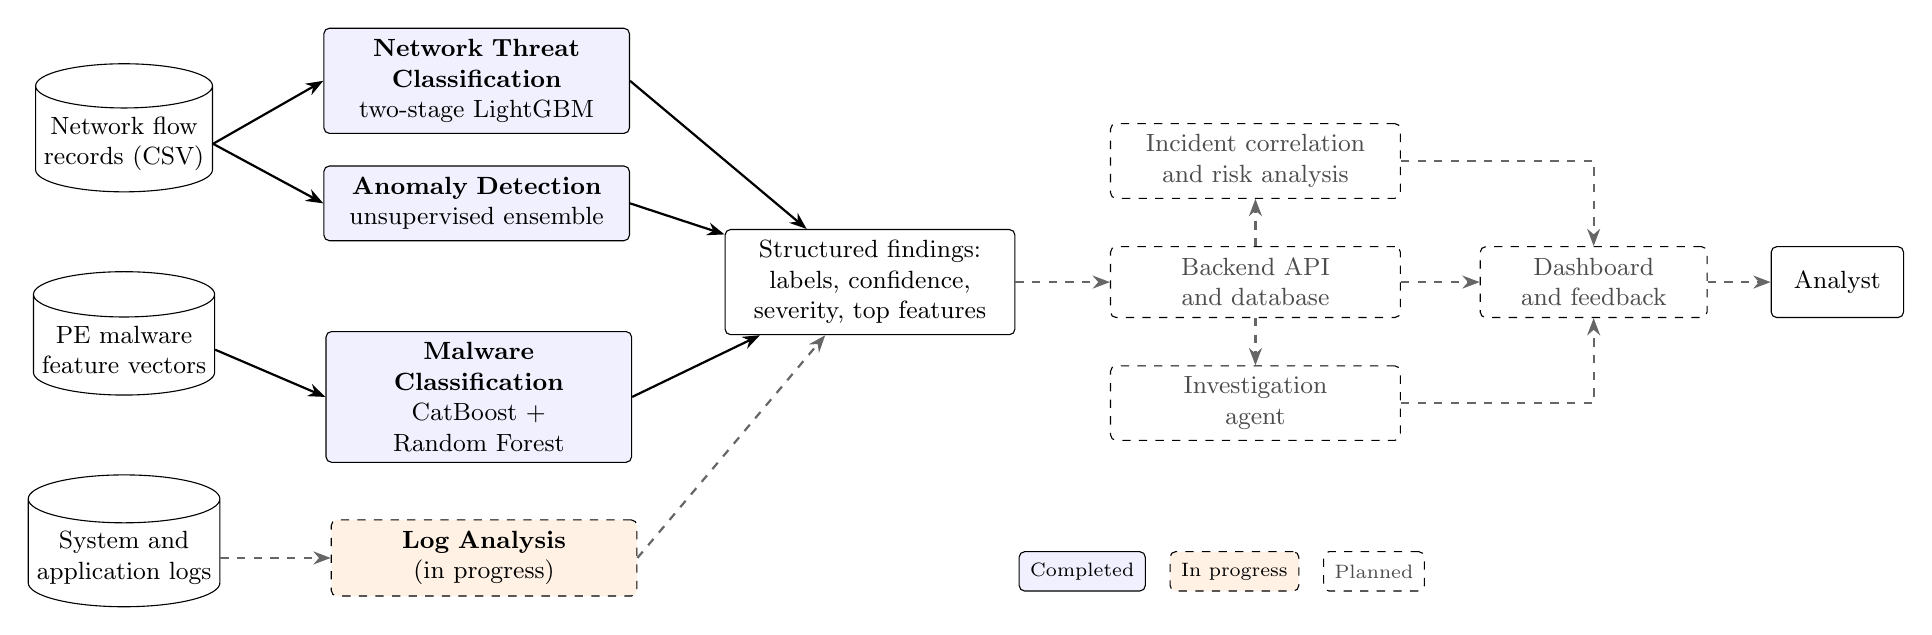
\begin{tikzpicture}[node distance=6mm and 8mm]
  % inputs
  \node[data] (flows) {Network flow\\records (CSV)};
  \node[data, below=10mm of flows] (pe) {PE malware\\feature vectors};
  \node[data, below=10mm of pe] (logs) {System and\\application logs};
  % modules
  \node[done, right=14mm of flows, yshift=8mm, text width=36mm] (ntc) {\textbf{Network Threat}\\\textbf{Classification}\\two-stage LightGBM};
  \node[done, below=4mm of ntc, text width=36mm] (ad) {\textbf{Anomaly Detection}\\unsupervised ensemble};
  \node[done, right=14mm of pe, yshift=-6mm, text width=36mm] (mw) {\textbf{Malware}\\\textbf{Classification}\\CatBoost + Random Forest};
  \node[wip, right=14mm of logs, text width=36mm] (log) {\textbf{Log Analysis}\\(in progress)};
  \draw[arr] (flows.east) -- (ntc.west);
  \draw[arr] (flows.east) -- (ad.west);
  \draw[arr] (pe.east) -- (mw.west);
  \draw[darr] (logs.east) -- (log.west);
  % outputs
  \node[box, right=12mm of ad, yshift=-10mm, text width=34mm] (out) {Structured findings:\\labels, confidence,\\severity, top features};
  \draw[arr] (ntc.east) -- (out);
  \draw[arr] (ad.east) -- (out);
  \draw[arr] (mw.east) -- (out);
  \draw[darr] (log.east) -- (out);
  % planned layer
  \node[plan, right=12mm of out, text width=34mm] (api) {Backend API\\and database};
  \node[plan, above=6mm of api, text width=34mm] (corr) {Incident correlation\\and risk analysis};
  \node[plan, below=6mm of api, text width=34mm] (agent) {Investigation\\agent};
  \node[plan, right=10mm of api, text width=26mm] (dash) {Dashboard\\and feedback};
  \node[box, right=8mm of dash, text width=14mm] (user) {Analyst};
  \draw[darr] (out) -- (api);
  \draw[darr] (api) -- (corr);
  \draw[darr] (api) -- (agent);
  \draw[darr] (corr.east) -| (dash.north);
  \draw[darr] (agent.east) -| (dash.south);
  \draw[darr] (api) -- (dash);
  \draw[darr] (dash) -- (user);
  % legend
  \node[done, below=14mm of agent, xshift=-22mm, minimum height=5mm, font=\scriptsize] (l1) {Completed};
  \node[wip, right=3mm of l1, minimum height=5mm, font=\scriptsize] (l2) {In progress};
  \node[plan, right=3mm of l2, minimum height=5mm, font=\scriptsize] (l3) {Planned};
\end{tikzpicture}}
\caption{Overall architecture of the AI-Based Autonomous Cyber Defense System and implementation status at mid-term}
\label{fig:architecture}
\end{figure}

The three completed modules do not yet exchange data with each other. They were developed independently, each by one team member, and they share a design principle: every module produces machine-readable output that the planned backend can consume. The network and anomaly modules both analyse flow records but answer different questions. The network module asks \textit{which known attack does this flow resemble?}, while the anomaly module asks \textit{how unusual is this flow compared with normal traffic?} Section~\ref{sec:module-relationship} discusses how the two are expected to complement each other.

\subsection{Module 1: Network Threat Classification}

\textbf{Role.} This module labels network flows as benign or as one of six attack families, so that the analyst sees what kind of activity is taking place, not just that something is wrong.

\textbf{Dataset.} The module uses the CIC-IDS2017 dataset published by the Canadian Institute for Cybersecurity \cite{sharafaldin2018cicids,cicids2017web}. It contains five days of benign and attack traffic, recorded as flows by the CICFlowMeter tool. All eight flow files were used, giving 2,830,743 usable flows described by 77 numeric features. Source and destination addresses, ports and timestamps were excluded so that the model cannot rely on identifiers. The original labels were grouped into seven classes (Table~\ref{tab:ntc-data}). In the module's taxonomy, the \textit{WebAttack} group also contains the FTP-Patator and SSH-Patator brute-force attacks and the Heartbleed exploit. The data is highly imbalanced: about 80.3\% of flows are benign, and only 36 Infiltration flows exist in the entire dataset.

\begin{table}[H]
\centering
\caption{Class distribution of the prepared CIC-IDS2017 data used by the Network Threat Classification module}
\label{tab:ntc-data}
\small
\begin{tabular}{lrrr}
\toprule
\textbf{Class} & \textbf{All rows} & \textbf{Train rows} & \textbf{Test rows} \\
\midrule
BENIGN       & 2,273,097 & 1,826,507 & 446,590 \\
DoS          &   252,661 &   206,951 &  45,710 \\
PortScan     &   158,930 &   129,834 &  29,096 \\
DDoS         &   128,027 &   102,360 &  25,667 \\
WebAttack    &    16,026 &    13,048 &   2,978 \\
Botnet       &     1,966 &     1,582 &     384 \\
Infiltration &        36 &        29 &       7 \\
\midrule
Total        & 2,830,743 & 2,280,311 & 550,432 \\
\bottomrule
\end{tabular}
\end{table}

\textbf{Method.} Preprocessing converts all features to numbers, replaces infinite values, imputes missing values with the training median, removes low-variance features and applies robust scaling. Each step is fitted on training data only, to avoid information leakage. The split keeps identical feature vectors in the same partition, using a fingerprint of selected flow fields. The classifier is a two-stage cascade of LightGBM gradient-boosted tree models \cite{ke2017lightgbm} (Figure~\ref{fig:ntc-flow}). Stage~1 decides between benign and attack, using a decision threshold of 0.7723 chosen on a validation subset. Flows predicted as attacks pass to Stage~2, which assigns one of the six families. Both models use balanced class weights instead of oversampling. Their settings are a learning rate of 0.05, 31 leaves, a minimum of 30 samples per leaf, 85\% feature and row sampling, and L1 and L2 regularisation of 0.1 and 2.0. Early stopping on a validation subset selected 600 trees for Stage~1, which is the configured maximum, and 256 trees for Stage~2. The module also attaches an Isolation Forest anomaly score, a feature-importance explanation, MITRE ATT\&CK context \cite{strom2018attack} and a recommended response plan to each decision. The response plan is produced as text only and is never executed.

\begin{figure}[H]
\centering
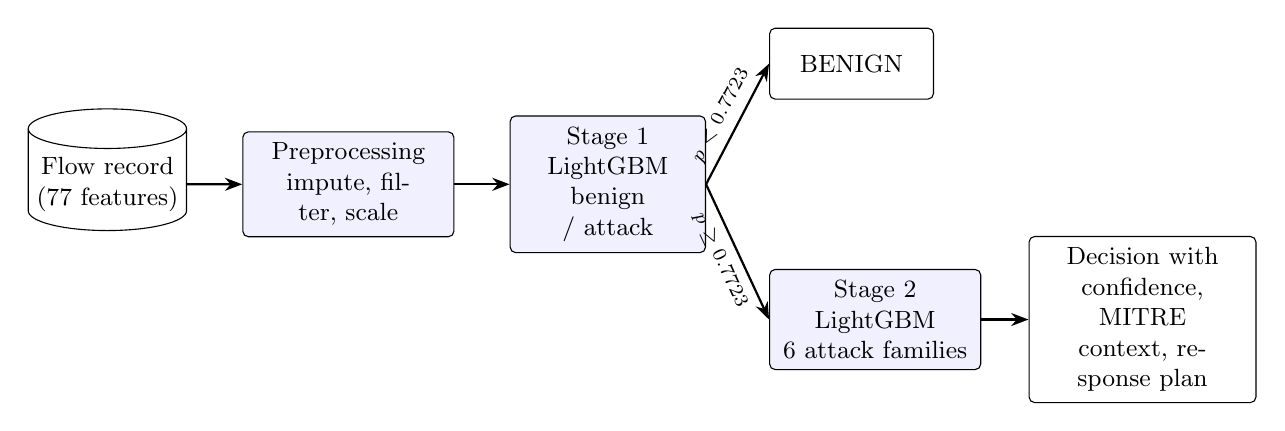
\begin{tikzpicture}[node distance=5mm and 7mm, every node/.style={font=\small}]
  \node[data] (in) {Flow record\\(77 features)};
  \node[done, right=of in, text width=24mm] (pre) {Preprocessing\\impute, filter, scale};
  \node[done, right=of pre, text width=22mm] (s1) {Stage 1\\LightGBM\\benign / attack};
  \node[box, above right=2mm and 8mm of s1, text width=18mm] (ben) {BENIGN};
  \node[done, below right=2mm and 8mm of s1, text width=24mm] (s2) {Stage 2\\LightGBM\\6 attack families};
  \node[box, right=6mm of s2, text width=26mm] (out) {Decision with\\confidence, MITRE\\context, response plan};
  \draw[arr] (in) -- (pre);
  \draw[arr] (pre) -- (s1);
  \draw[arr] (s1.east) -- node[above, font=\scriptsize, sloped] {$p<0.7723$} (ben.west);
  \draw[arr] (s1.east) -- node[below, font=\scriptsize, sloped] {$p\geq0.7723$} (s2.west);
  \draw[arr] (s2) -- (out);
\end{tikzpicture}
\caption{Two-stage workflow of the Network Threat Classification module}
\label{fig:ntc-flow}
\end{figure}

\textbf{Results.} The cascade was evaluated once on the 550,432-flow holdout set (Table~\ref{tab:ntc-results}). The binary gate reached 99.70\% attack precision and 99.84\% attack recall. Of the 446,590 benign test flows, 313 were wrongly flagged, and of the 103,842 attack flows, 164 were missed. The end-to-end cascade achieved 99.91\% accuracy with a macro F1-score of 0.9578. The gap between this value and the weighted F1-score of 0.9991 reflects weaker results on rare classes. Botnet recall is 71.35\% (274 of 384 test flows), and the Infiltration result of six correct out of seven is too small to be statistically reliable. Figure~\ref{fig:ntc-cm} shows the confusion matrices.

\begin{table}[H]
\centering
\caption{Holdout performance of the Network Threat Classification module (CIC-IDS2017)}
\label{tab:ntc-results}
\small
\begin{tabular}{lrrrr}
\toprule
\textbf{Evaluation} & \textbf{Rows} & \textbf{Accuracy} & \textbf{Macro F1} & \textbf{Weighted F1} \\
\midrule
Stage 1 (benign vs.\ attack) & 550,432 & 99.91\% & 0.9986 & 0.9991 \\
Stage 2 on true attacks only & 103,842 & 99.98\% & 0.9997 & 0.9998 \\
End-to-end cascade & 550,432 & 99.91\% & 0.9578 & 0.9991 \\
\bottomrule
\end{tabular}
\end{table}

\begin{figure}[htbp]
\centering
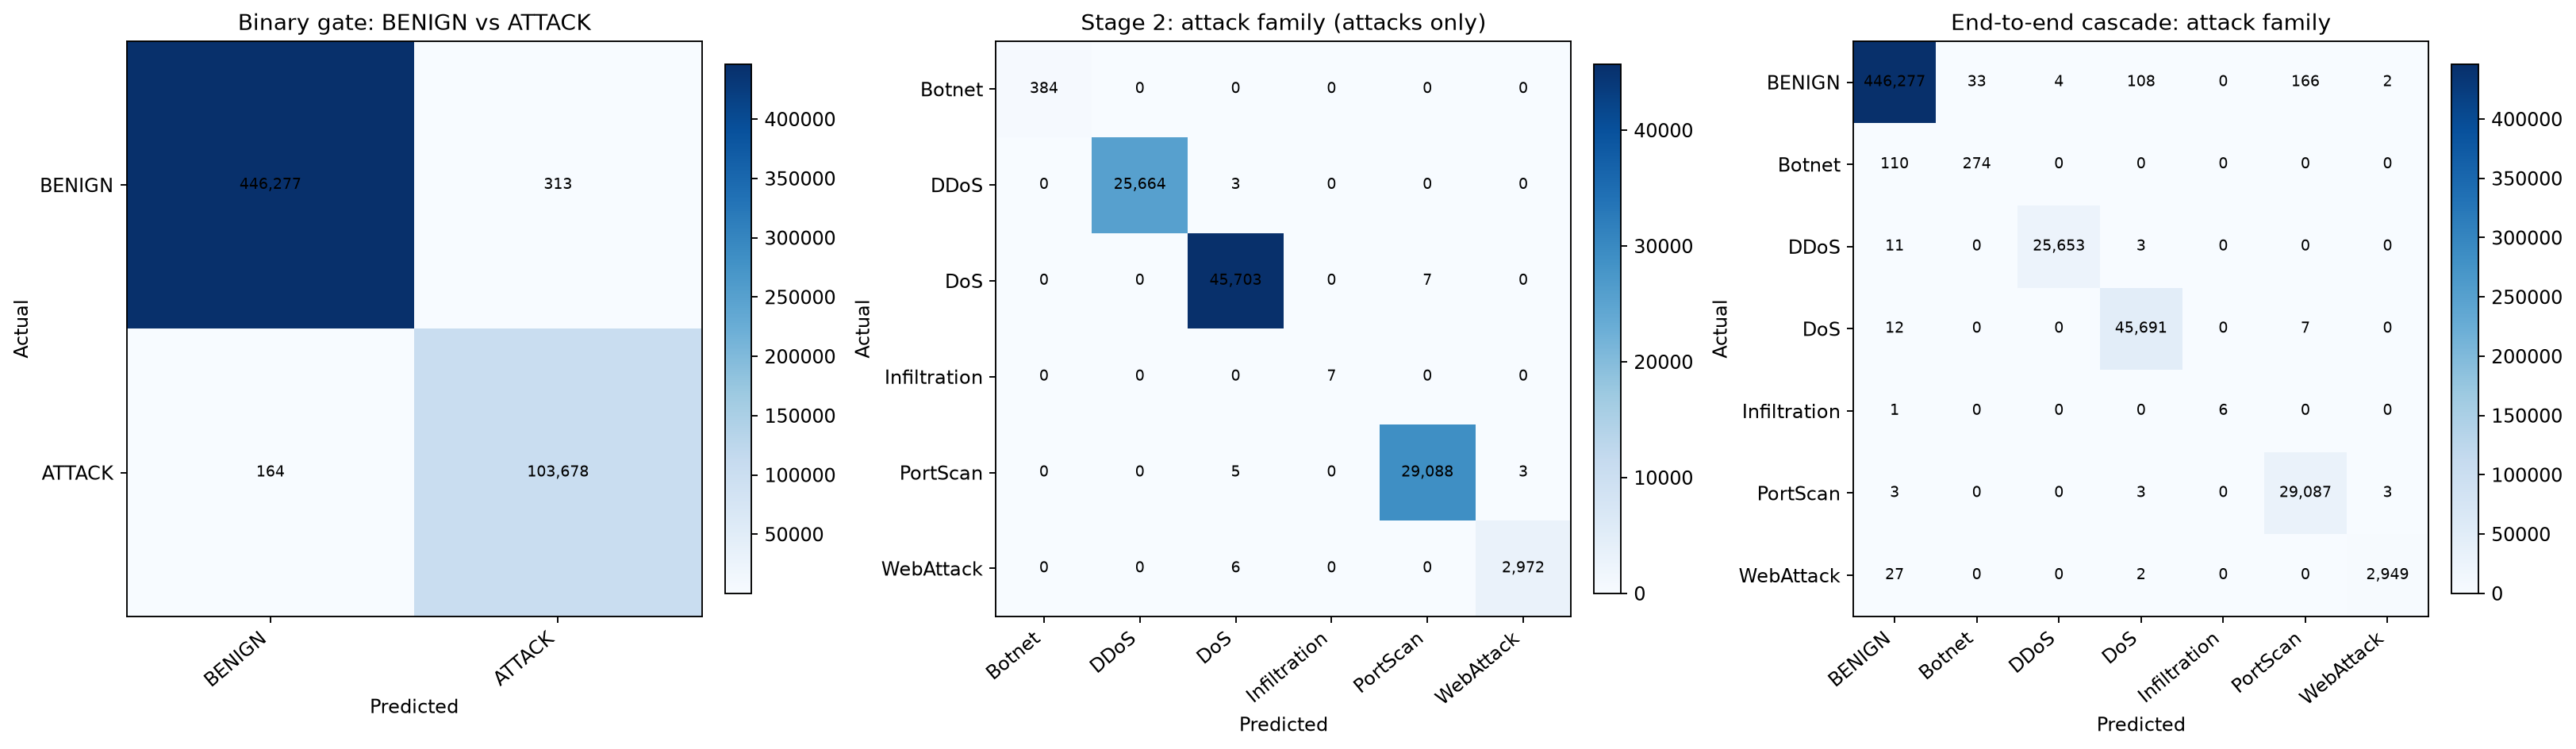
\includegraphics[width=\textwidth]{ntc_eda_4.png}
\caption{Confusion matrices of the Network Threat Classification module on the holdout set: binary gate (left), Stage~2 on true attacks (centre) and end-to-end cascade (right)}
\label{fig:ntc-cm}
\end{figure}

\textbf{Limitations.} CIC-IDS2017 was recorded in a single laboratory network over five days, so these results do not show how the model would perform on a different network or on future traffic. Previous work has also reported labelling and flow-construction problems in this dataset \cite{engelen2021troubleshooting}. The rare classes (Botnet and Infiltration) have too few examples for reliable estimates. Stage~1 used the maximum number of trees allowed, so a wider search might improve it. The attached Isolation Forest score has not been validated against labelled data and is not presented as a detector of new attacks. The current interface is a command-line tool and Python API; live packet capture and response execution are outside the verified scope.

\subsection{Module 2: Malware Classification}

\textbf{Role.} This module decides whether a Windows executable is benign or malicious and, if it is malicious, which category of malware it belongs to. This tells the analyst both whether a file is dangerous and what kind of behaviour to expect from it.

\textbf{Dataset.} The module uses BODMAS, a dataset of Windows PE samples released for research on learning-based malware analysis \cite{yang2021bodmas}. The cleaned version used contains 134,428 samples (77,138 benign and 57,290 malicious), each described by 2,326 numerical static features. The feature format follows the EMBER feature set \cite{anderson2018ember}. Category labels were joined to the malicious samples, and eight categories were selected for the second stage (Table~\ref{tab:mw-data}). Very small categories were left out.

\begin{table}[H]
\centering
\caption{Malware categories used by the second stage of the Malware Classification module (BODMAS)}
\label{tab:mw-data}
\small
\begin{tabular}{lr@{\hspace{3em}}lr}
\toprule
\textbf{Category} & \textbf{Samples} & \textbf{Category} & \textbf{Samples} \\
\midrule
Trojan     & 29,972 & Ransomware          & 821 \\
Worm       & 16,695 & Dropper             & 715 \\
Backdoor   &  7,331 & Information stealer & 447 \\
Downloader &  1,031 & Virus               & 192 \\
\bottomrule
\end{tabular}
\end{table}

\textbf{Method.} Both stages use a stratified 80/20 train--test split with a fixed random seed of 42 (Figure~\ref{fig:mw-flow}). No feature scaling is applied, which suits tree-based models, and no synthetic oversampling such as SMOTE was used. Stage~1 is a CatBoost gradient-boosting classifier \cite{prokhorenkova2018catboost} with 300 iterations, depth 6 and a learning rate of 0.1. Stage~2 is a Random Forest \cite{breiman2001rf} with 100 trees, square-root feature sampling, at least two samples per leaf, and \texttt{balanced\_subsample} class weighting to reduce the effect of category imbalance. A Gradio interface \cite{abid2019gradio} loads the saved models, accepts a CSV file containing the 2,326 features, and displays predictions, confusion matrices and summary charts.

\begin{figure}[H]
\centering
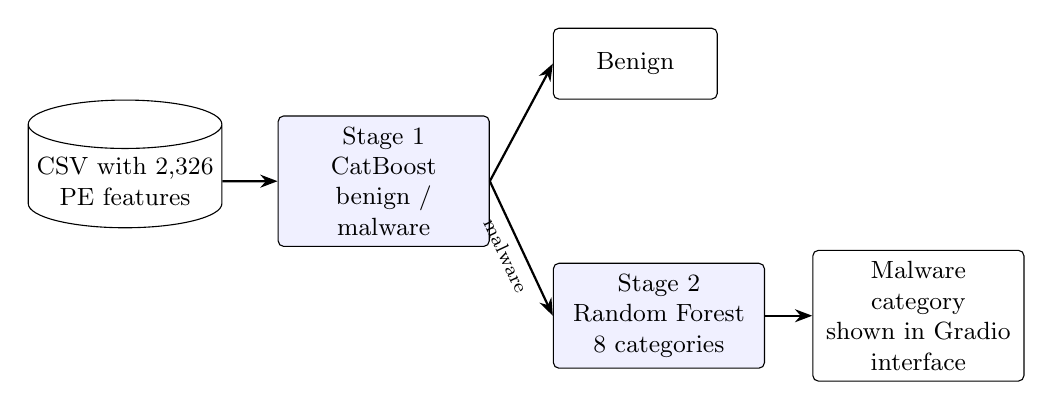
\begin{tikzpicture}[node distance=5mm and 7mm, every node/.style={font=\small}]
  \node[data] (in) {CSV with 2,326\\PE features};
  \node[done, right=of in, text width=24mm] (s1) {Stage 1\\CatBoost\\benign / malware};
  \node[box, above right=2mm and 8mm of s1, text width=18mm] (ben) {Benign};
  \node[done, below right=2mm and 8mm of s1, text width=24mm] (s2) {Stage 2\\Random Forest\\8 categories};
  \node[box, right=6mm of s2, text width=24mm] (out) {Malware category\\shown in Gradio\\interface};
  \draw[arr] (in) -- (s1);
  \draw[arr] (s1.east) -- (ben.west);
  \draw[arr] (s1.east) -- node[below, font=\scriptsize, sloped] {malware} (s2.west);
  \draw[arr] (s2) -- (out);
\end{tikzpicture}
\caption{Two-stage workflow of the Malware Classification module}
\label{fig:mw-flow}
\end{figure}

\textbf{Results.} Table~\ref{tab:mw-results} lists the results reported in the module's documentation. On the 26,886-sample test set, the CatBoost detector misclassified 62 benign samples as malware and missed 71 malicious samples. The Random Forest category classifier reached 94.34\% accuracy and a macro F1-score of 0.8766. The lower macro value reflects weaker results on small categories, especially Virus, which has only 192 samples in the whole dataset.

\begin{table}[H]
\centering
\caption{Test results of the Malware Classification module (as reported in the module documentation)}
\label{tab:mw-results}
\small
\begin{tabular}{llr}
\toprule
\textbf{Stage} & \textbf{Metric} & \textbf{Value} \\
\midrule
\multirow{5}{*}{Stage 1: CatBoost (benign vs.\ malware)}
 & Accuracy              & 99.51\% \\
 & Precision (malware)   & 99.46\% \\
 & Recall (malware)      & 99.38\% \\
 & F1-score (malware)    & 99.42\% \\
 & ROC-AUC               & 99.97\% \\
\midrule
\multirow{3}{*}{Stage 2: Random Forest (8 categories)}
 & Accuracy              & 94.34\% \\
 & Macro F1-score        & 87.66\% \\
 & Weighted F1-score     & 94.32\% \\
\bottomrule
\end{tabular}
\end{table}

\textbf{Limitations.} The module classifies pre-extracted feature vectors. It does not yet extract features from raw executable files, scan endpoints in real time, or quarantine files. The Stage~2 result was measured on samples already known to be malicious, so it shows how well categories are separated, not the error of the full two-stage pipeline. The two stages were also evaluated on separate splits. Metrics from earlier experiments, such as a CatBoost run with 99.00\% accuracy, are not part of the final pipeline. The values in Table~\ref{tab:mw-results} must be re-confirmed against the saved metrics file before the final report. Finally, malware evolves over time, and a random split may overestimate performance on future samples. Temporal evaluation, which BODMAS was designed to support \cite{yang2021bodmas}, is left for future work.

\subsection{Module 3: Anomaly Detection}

\textbf{Role.} This module detects network activity that deviates from normal behaviour, whether or not it matches a known attack. It is trained only on benign traffic, so it needs no attack labels to learn and can flag attack types that the supervised classifiers have never seen \cite{chandola2009anomaly,ahmed2016anomaly}. Each alert includes a severity level and the features that were most abnormal, so that the analyst can see why it was raised.

\textbf{Datasets and protocol.} The module was evaluated on NSL-KDD \cite{tavallaee2009nslkdd} and CIC-IDS2017 \cite{sharafaldin2018cicids}. NSL-KDD uses its official training and test files. Its test file contains 17 attack types (3,750 of 12,833 attack records) that never appear in training, which makes it a direct test of detecting unseen attacks. For CIC-IDS2017, an analysis found that 10.9\% of all rows (23.6\% of attack rows) are exact duplicates, and 1,396 rows have identical features but conflicting labels. Duplicate flows split across training and test sets would inflate results. The module therefore removes duplicates and conflicting rows before splitting, then draws a fixed 10\% sample and splits it 70/30 with stratification (176,467 training and 75,630 test flows). All design choices were made on a validation split carved from the training data. The test sets were used only for the final measurements, which are averaged over three random seeds.

\textbf{Method.} The pipeline is shown in Figure~\ref{fig:ad-flow}:
\begin{itemize}[itemsep=1pt, topsep=2pt]
  \item \textbf{Preprocessing}, fitted on benign training data: median imputation, a signed logarithmic transform for heavy-tailed counts, one-hot encoding, robust scaling, and, for CIC-IDS2017, removal of features with absolute correlation above 0.99 with an already kept feature (70 reduced to 48 features).
  \item \textbf{Detectors.} Four unsupervised detectors are available: an Isolation Forest \cite{liu2008iforest}, the Local Outlier Factor (LOF) \cite{breunig2000lof}, an autoencoder that scores flows by reconstruction error \cite{hinton2006autoencoder}, and a robust z-score baseline.
  \item \textbf{Score combination.} Each detector's score is converted to its rank among the scores of held-out benign traffic, and the selected detectors are combined.
  \item \textbf{Threshold.} An alert is raised when the combined score exceeds a percentile of the benign scores.
\end{itemize}

\begin{figure}[H]
\centering
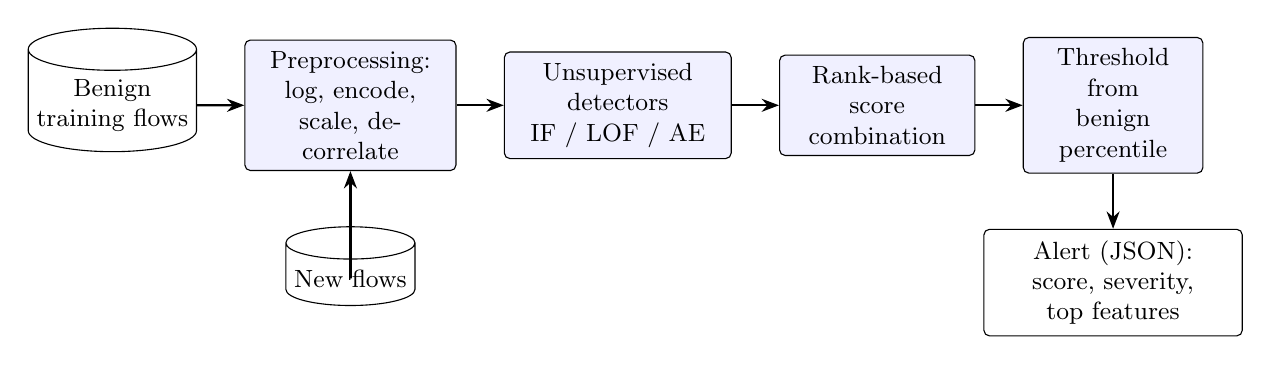
\begin{tikzpicture}[node distance=5mm and 6mm, every node/.style={font=\small}]
  \node[data] (in) {Benign\\training flows};
  \node[done, right=of in, text width=24mm] (pre) {Preprocessing:\\log, encode,\\scale, de-correlate};
  \node[done, right=of pre, text width=26mm] (det) {Unsupervised\\detectors\\IF / LOF / AE};
  \node[done, right=of det, text width=22mm] (ens) {Rank-based\\score\\combination};
  \node[done, right=of ens, text width=20mm] (thr) {Threshold from\\benign\\percentile};
  \node[box, below=7mm of thr, text width=30mm] (al) {Alert (JSON):\\score, severity,\\top features};
  \node[data, below=7mm of pre] (new) {New flows};
  \draw[arr] (in) -- (pre);
  \draw[arr] (pre) -- (det);
  \draw[arr] (det) -- (ens);
  \draw[arr] (ens) -- (thr);
  \draw[arr] (thr) -- (al);
  \draw[arr] (new) -| (pre);
\end{tikzpicture}
\caption{Workflow of the Anomaly Detection module}
\label{fig:ad-flow}
\end{figure}

The first version (v1) averaged all four detectors and used a fixed 99th-percentile threshold. Its evaluation exposed clear weaknesses. On CIC-IDS2017 it detected only 3.9\% of attacks, because weak detectors diluted the combined score and the threshold was too strict. An improved version (v2) was then tuned in stages, entirely on validation data:
\begin{enumerate}[itemsep=1pt, topsep=2pt]
  \item removing redundant features;
  \item a grid search over each detector's settings;
  \item a search over all 60 combinations of detector subset, normalisation and combination rule;
  \item selection of the alert percentile by F1-score.
\end{enumerate}
A change was adopted only if it improved the validation result. Table~\ref{tab:ad-config} shows the selected configurations. A \textit{hybrid} variant was also evaluated. It adds a supervised Random Forest \cite{breiman2001rf} for known attacks and flags a flow if either part flags it.

\begin{table}[H]
\centering
\caption{Configuration of the improved (v2) anomaly detector selected on validation data}
\label{tab:ad-config}
\small
\begin{tabular}{P{0.3\textwidth}P{0.3\textwidth}P{0.3\textwidth}}
\toprule
\textbf{Setting} & \textbf{NSL-KDD} & \textbf{CIC-IDS2017} \\
\midrule
Detectors combined & Isolation Forest + LOF & LOF + autoencoder \\
Combination rule & maximum of ranks & mean of ranks \\
LOF & 10 neighbours, 30,000 reference flows & 10 neighbours, 30,000 reference flows \\
Isolation Forest & 4,096 samples per tree, 50\% of features & (not used) \\
Autoencoder & (not used) & up to 200 epochs, early stopping \\
Alert threshold & 95th percentile & 97th percentile \\
\bottomrule
\end{tabular}
\end{table}

\textbf{Results.} Table~\ref{tab:ad-results} compares the original detector, the improved detector and the hybrid on the untouched test sets. On CIC-IDS2017, the improved detector raised the F1-score from 0.071 to 0.835 and the PR-AUC from 0.534 to 0.891, while raising the false-positive rate from 0.9\% to 2.9\%. On NSL-KDD the F1-score rose from 0.522 to 0.899, but this gain came mainly from a lower threshold. The false-positive rate rose from 5.5\% to 11.9\%, and the threshold-independent PR-AUC was about 0.01 lower than v1. The most important result for the platform concerns unseen attacks. On the 17 NSL-KDD attack types absent from training, recall rose from 41.2\% (v1) to 84.5\% (v2) at seed 42. The hybrid's supervised part added almost nothing there (85.1\%), as expected, since a supervised model cannot recognise new attack types. Figure~\ref{fig:ad-results} shows the CIC-IDS2017 comparison.

\begin{table}[H]
\centering
\caption{Anomaly Detection test results: original (v1), improved (v2) and hybrid (mean of three seeds)}
\label{tab:ad-results}
\small
\begin{tabular}{llrrrr}
\toprule
\textbf{Dataset} & \textbf{Model} & \textbf{F1-score} & \textbf{Recall} & \textbf{False-positive rate} & \textbf{PR-AUC} \\
\midrule
\multirow{3}{*}{NSL-KDD} & Original (v1) & 0.522 & 36.9\% & 5.5\%  & 0.911 \\
                         & Improved (v2) & 0.899 & 89.1\% & 11.9\% & 0.901 \\
                         & Hybrid        & 0.904 & 90.0\% & 12.1\% & 0.956 \\
\midrule
\multirow{3}{*}{CIC-IDS2017} & Original (v1) & 0.071 & 3.9\%  & 0.9\% & 0.534 \\
                             & Improved (v2) & 0.835 & 82.2\% & 2.9\% & 0.891 \\
                             & Hybrid        & 0.931 & 99.7\% & 3.0\% & 0.998 \\
\bottomrule
\end{tabular}
\end{table}

\begin{figure}[htbp]
\centering
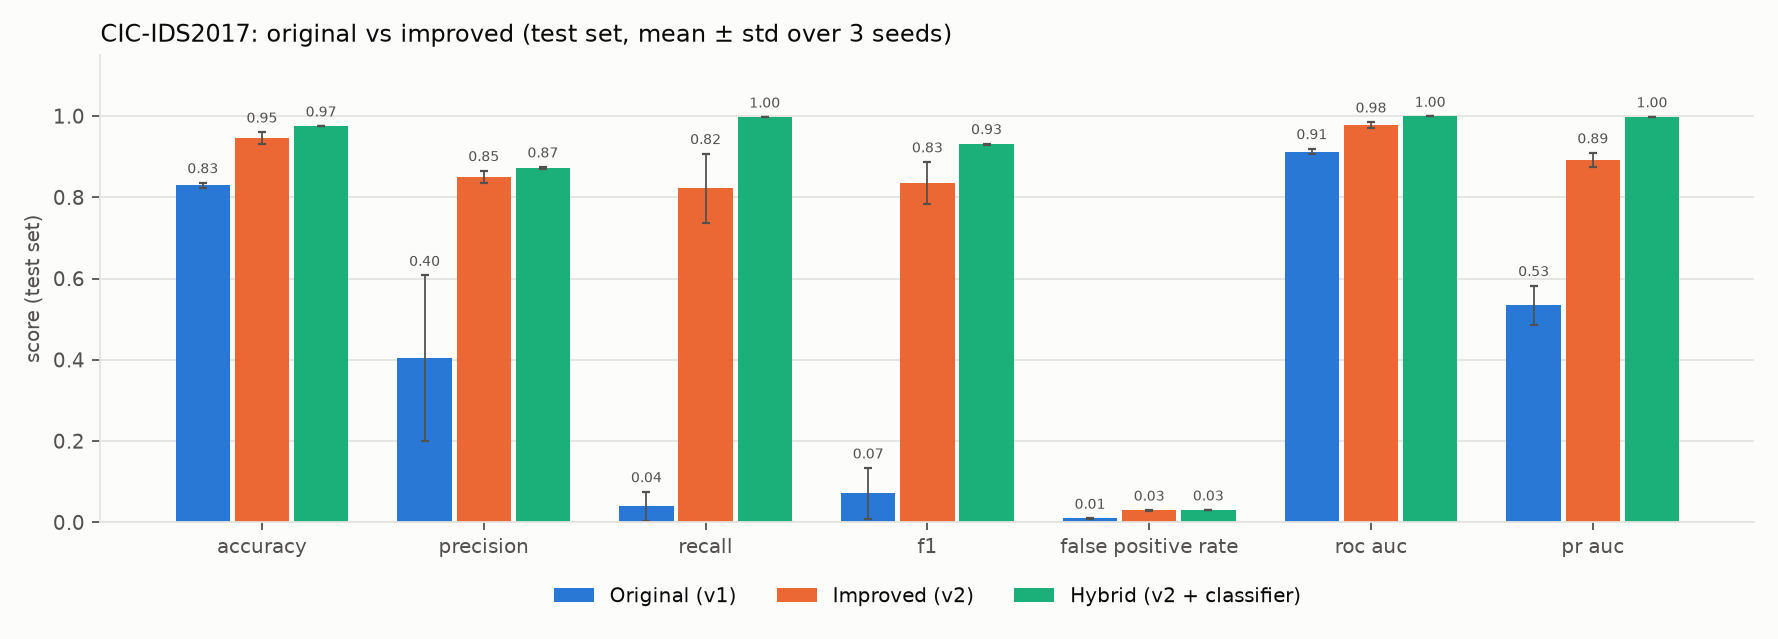
\includegraphics[width=\textwidth]{anomaly_cic_comparison.png}
\caption{Anomaly Detection on CIC-IDS2017: original vs.\ improved vs.\ hybrid (test set, mean $\pm$ standard deviation over three seeds)}
\label{fig:ad-results}
\end{figure}

\textbf{Limitations.} The rise in false positives on NSL-KDD comes from a known difference between the normal traffic in its training and test files. The training false-positive rate was 4.6\%, against 11.8\% on test, so thresholds will need recalibration on each deployment network. On CIC-IDS2017, the v2 detector still rarely detects SSH-Patator, web attacks and Bot traffic, which look statistically similar to normal flows. The F1-score of v2 on CIC-IDS2017 varied between 0.776 and 0.876 across seeds. Tuning used a single validation split instead of cross-validation. Before this protocol was fixed, an early exploratory analysis had examined CIC-IDS2017 test results; this is disclosed as a possible source of bias.

\subsection{Relationship Between the Modules}
\label{sec:module-relationship}

The three modules address different parts of the same defensive task. Network Threat Classification and Malware Classification are supervised. They are precise on the attack families and malware categories present in their training data, but they cannot recognise genuinely new behaviour. Anomaly Detection is unsupervised, so it is less precise but can flag behaviour that has never been labelled. The anomaly module's evaluation supports this division of labour: its supervised component lifted recall on known CIC-IDS2017 attacks from 82\% to 99.7\%, while on unseen NSL-KDD attacks the unsupervised detector provided almost all of the coverage. In the integrated system, the network classifier is expected to take the supervised role for flows and the anomaly detector the unsupervised role, and their outputs will be combined by the planned correlation component. This combination has not yet been implemented or tested.

Two points must be kept in mind when comparing the modules. First, the network classifier also produces an Isolation Forest anomaly score. That score is an unvalidated auxiliary signal, whereas the Anomaly Detection module is the dedicated, evaluated component for this task. Second, both flow modules use CIC-IDS2017 but with different protocols. The network module keeps duplicate flows (grouped within one partition) and uses the full dataset, while the anomaly module removes duplicates and uses a 10\% sample. Their numbers are therefore not directly comparable, and the integration phase will need a common evaluation split.

\subsection{Planned Components}

Table~\ref{tab:status} summarises the implementation status of all proposed components. Log analysis is under development. The backend API and database (FastAPI and a relational database are planned), the dashboard (React is planned), incident correlation, risk analysis and the investigation agent will be developed in later increments. The agent will follow the main steps of incident handling described in NIST guidance \cite{nist80061r3}.

\begin{table}[H]
\centering
\caption{Implementation status of the proposed components at mid-term}
\label{tab:status}
\small
\begin{tabular}{lll}
\toprule
\textbf{Component} & \textbf{Status} & \textbf{Current form} \\
\midrule
Network Threat Classification & Completed & Prototype; CLI and Python API \\
Malware Classification & Completed & Prototype; Gradio interface \\
Anomaly Detection & Completed & Prototype; CLI and Python API \\
Log Analysis & In progress & Under development \\
Network Monitoring (live capture) & Planned & -- \\
Incident Correlation & Planned & -- \\
Vulnerability Analysis & Planned & -- \\
Attack-Path Analysis & Planned & -- \\
Attack Prediction & Planned & -- \\
Risk Analysis & Planned & -- \\
Investigation Agent & Planned & -- \\
Dashboard and Feedback & Planned & -- \\
Integration backend and database & Planned & -- \\
\bottomrule
\end{tabular}
\end{table}

\subsection{Design Considerations}

\textbf{User interface and experience.} The planned dashboard will group alerts into incidents and show, for each one, the module that raised it, its severity, its confidence and the features behind it. The aim is that an analyst can understand an alert without opening several tools. The Gradio interface of the malware module is an early example of this approach.

\textbf{Technical implementation.} All modules are implemented in Python with widely used libraries, and each saves its trained models and preprocessing objects so that it can be reloaded for inference without retraining. The planned backend will expose each module through a common interface, so that adding or replacing a model does not affect the others.

\textbf{Security and data privacy.} The modules are trained only on public datasets and store no personal data. In a deployment, flow records and logs may contain sensitive information, so the planned backend will need access control, and stored results will need protection. The decision to produce response recommendations instead of executing them is also a safety measure, since an incorrect automatic block could disrupt legitimate services.

\textbf{Customisation and flexibility.} Thresholds, detector choices and model settings are kept in configuration files rather than in code. The anomaly module, for example, stores its tuned settings for each dataset in YAML files. An organisation can therefore adjust its false-alarm budget or retrain a module on its own data.

\textbf{Anticipated impact.} The completed modules show that the platform can give specific labels for known network attacks and malware, and can still flag a large share of previously unseen attacks. Once integrated, these results should reduce the time analysts spend on initial triage, provided that the models are validated on the target network first.

\section{Software Process Model}

A software process model is a structured description of the activities used to develop a system, such as requirements analysis, design, implementation, testing and deployment, and of the order in which they are carried out \cite{sommerville2016se}. Common models include the Waterfall model, in which phases follow one another strictly; Agile methods, which work in short, flexible iterations; the Spiral model, which focuses on risk; and the Incremental model, in which the system is delivered as a series of increments, each adding working functionality \cite{sommerville2016se,larman2003iterative}.

\textbf{Chosen model.} The project follows the \textbf{Incremental model}. The system is divided into parts that are specified, built and tested in separate increments, each producing working functionality that later increments extend. Within each increment, the usual activities of analysis, design, implementation and testing are carried out in sequence (Figure~\ref{fig:process}).

\textbf{Justification.}
\begin{itemize}[itemsep=1pt, topsep=2pt]
  \item \textit{Project complexity.} The proposed system has twelve modules. Building them all at once would be risky; developing them in increments allows each to be finished and evaluated before the next is started.
  \item \textit{Team structure.} The first increment could be divided naturally among the three team members, each responsible for one analysis module. This is how the network, malware and anomaly modules were developed in parallel.
  \item \textit{Flexibility.} Results from one increment inform the next. For example, the anomaly module's evaluation exposed duplicate records in CIC-IDS2017 and the need for recalibrated thresholds, and these findings will shape the integration work.
  \item \textit{Timeline.} The academic calendar requires demonstrable progress at mid-term. The Incremental model guarantees that a tested subset of the system exists at that point.
\end{itemize}

\begin{figure}[htbp]
\centering
\resizebox{\textwidth}{!}{%
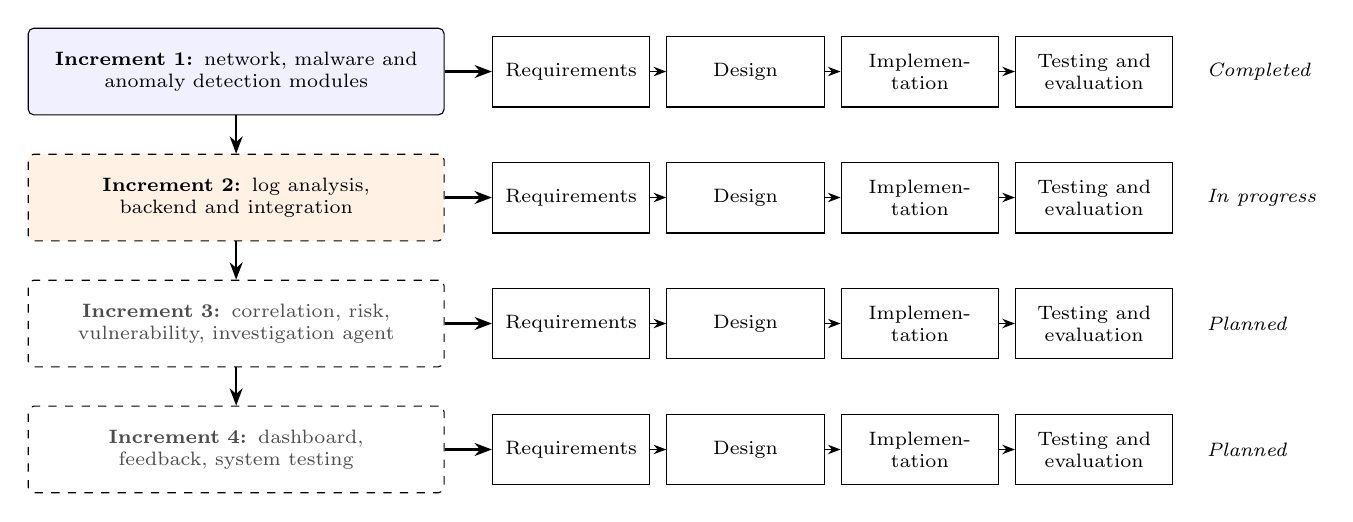
\begin{tikzpicture}[every node/.style={font=\small}]
  \tikzset{ph/.style={draw, minimum width=20mm, minimum height=9mm, align=center, font=\scriptsize},
           inc/.style={text width=50mm, minimum height=11mm, font=\scriptsize}}
  \node[done, inc, anchor=west] (inc1) at (0,0)      {\textbf{Increment 1:} network, malware and\\anomaly detection modules};
  \node[wip,  inc, anchor=west] (inc2) at (0,-16mm)  {\textbf{Increment 2:} log analysis,\\backend and integration};
  \node[plan, inc, anchor=west] (inc3) at (0,-32mm)  {\textbf{Increment 3:} correlation, risk,\\vulnerability, investigation agent};
  \node[plan, inc, anchor=west] (inc4) at (0,-48mm)  {\textbf{Increment 4:} dashboard,\\feedback, system testing};
  \foreach \i/\lab in {1/Completed, 2/In progress, 3/Planned, 4/Planned} {
    \node[ph, right=6mm of inc\i] (r\i) {Requirements};
    \node[ph, right=2mm of r\i] (d\i) {Design};
    \node[ph, right=2mm of d\i] (c\i) {Implemen-\\tation};
    \node[ph, right=2mm of c\i] (t\i) {Testing and\\evaluation};
    \node[right=3mm of t\i, font=\scriptsize\itshape, anchor=west] {\lab};
    \draw[arr] (inc\i) -- (r\i);
    \draw[-{Stealth[length=1.6mm]}] (r\i) -- (d\i);
    \draw[-{Stealth[length=1.6mm]}] (d\i) -- (c\i);
    \draw[-{Stealth[length=1.6mm]}] (c\i) -- (t\i);
  }
  \draw[arr] (inc1) -- (inc2);
  \draw[arr] (inc2) -- (inc3);
  \draw[arr] (inc3) -- (inc4);
\end{tikzpicture}}
\caption{Incremental development model applied to the project, with the status of each increment at mid-term}
\label{fig:process}
\end{figure}

\textbf{Stages within each increment.}
\begin{itemize}[itemsep=1pt, topsep=2pt]
  \item \textit{Requirements analysis.} The requirements for the increment are drawn from the proposal, the literature, dataset documentation and supervisor meetings (Section~3.4).
  \item \textit{Design.} Each module's data pipeline, model architecture and output format are designed. Integration increments also design the shared interfaces.
  \item \textit{Implementation.} Modules are implemented in Python and their trained models are saved for reuse.
  \item \textit{Testing and evaluation.} Each model is evaluated on held-out data with metrics suited to imbalanced classes. Code is checked with unit tests where available; the anomaly module, for example, has an automated test suite. Integration and system testing will be carried out in Increments 2--4.
  \item \textit{Deployment and maintenance.} Deployment is limited to a controlled demonstration environment. Maintenance consists of retraining models and recalibrating thresholds as new data becomes available.
\end{itemize}

\textbf{Advantages for this project.} Each increment ends with something that works and can be measured, so problems are found early. In Increment~1, for example, evaluation revealed weak results in the first version of the anomaly detector and duplicate data in CIC-IDS2017, and both were addressed before mid-term. Regular supervisor reviews at the end of each increment keep the work aligned with the project goals.

\textbf{Challenges and mitigation.} The main risk of incremental development is that independently built parts may be difficult to integrate later. Increment~1 has indeed produced three modules with different interfaces and data formats. This is mitigated by making integration the focus of Increment~2, before further modules are added, and by requiring every module to produce structured output.


\chapter{Software Requirements Specification}

A Software Requirements Specification (SRS) records what a software system must do and the qualities it must have. Functional requirements describe the behaviour the system provides, and non-functional requirements describe properties such as performance, reliability, usability and security \cite{sommerville2016se,iso29148}. A clear SRS gives all stakeholders a shared reference: developers know what to build, testers know what to verify, and supervisors can judge progress against agreed expectations. It also limits scope creep, because new ideas can be checked against what was actually agreed.

For a project developed in increments, the SRS also shows which requirements have already been met. This chapter introduces the document's scope and audience, lists the functional requirements of the implemented modules and the planned system with their current status, defines the non-functional requirements, describes the techniques used to gather the requirements, and presents the project time frame.

\section{Introduction}

This SRS describes the requirements of the AI-Based Autonomous Cyber Defense System. It guides the remaining development work and gives the team, the supervisor and the evaluation committee a common reference for what the system is expected to do. Because three modules are already implemented, the requirements in this chapter are of two kinds. Some describe behaviour that exists and has been tested on benchmark data. Others describe behaviour planned for later increments. Every requirement is labelled accordingly. The requirements were derived from the approved proposal and refined through the literature review, analysis of the datasets and their documentation, and regular supervisor meetings (Section~\ref{sec:req-gathering}).

\subsection{Document Scope}

The document covers both functional and non-functional requirements. The functional requirements state the inputs each module accepts, the processing it performs and the outputs it produces, together with the system-level functions planned for integration: storage, correlation, risk analysis, investigation support and the dashboard. The non-functional requirements set expectations for quality attributes, including accuracy, explainability, usability, maintainability and interoperability, as well as performance, safety, privacy and reproducibility. The SRS focuses on \textit{what} the system must do and \textit{why}. The internal design of the models is described in Chapter~2. Detailed design artefacts, such as use cases and sequence diagrams, belong to the next stage of the project.

\subsection{Audience}

The SRS is written for the following readers:

\begin{itemize}
    \setlength{\itemsep}{1pt}
    \setlength{\parskip}{0pt}
    \setlength{\parsep}{0pt}
    \item \textbf{Development team:} the three team members, who use the SRS to keep their modules consistent with each other and to plan the integration increment.
    \item \textbf{Supervisor and FYP committee:} who use it to assess the scope of the project and the progress made against agreed requirements.
    \item \textbf{Testing team:} in this project, the developers themselves, who derive unit, integration and system test cases from the listed requirements.
    \item \textbf{End users (security analysts and administrators):} whose needs, as identified in Chapter~1, are expressed in the functional and usability requirements.
    \item \textbf{Documentation team:} who use the SRS as the basis for user guides and the final report.
    \item \textbf{User experience designers:} who use the dashboard and feedback requirements to design the planned interface.
    \item \textbf{Future maintenance team:} who need to understand the expected behaviour of each module before retraining models or adding new ones.
\end{itemize}

\section{Functional Requirements}

Functional requirements define the services a system provides: the inputs it accepts, how it processes them and the outputs it returns \cite{sommerville2016se}. They are the basis for design, for test cases and for checking at the end of the project whether the system does what was agreed. Each requirement below is written to be specific enough to be tested.

Table~\ref{tab:FRs} lists the functional requirements, grouped by module. The \textit{Status} column shows the state at mid-term: \textbf{Done} means implemented and tested on benchmark data, \textbf{Partial} means implemented with a known limitation, \textbf{WIP} means in progress, and \textbf{Planned} means scheduled for a later increment.

{\footnotesize
\begin{center}
\begin{longtable}{p{0.15\textwidth}p{0.65\textwidth}p{0.08\textwidth}}
   \caption{\label{tab:FRs}Functional Requirements}\\
   \hline
   \hline
   \textbf{Requirement ID} & \textbf{Description} & \textbf{Status} \\
	\hline
\endfirsthead
\multicolumn{3}{l}%
{\tablename\ \thetable\ -- \textit{Continued from previous page}} \\
\hline
   \textbf{Requirement ID} & \textbf{Description} & \textbf{Status} \\
\hline
\endhead
\hline \multicolumn{3}{r}{\textit{Continued on next page}} \\
\endfoot
\hline
\endlastfoot

  \multicolumn{3}{l}{\textit{Network Threat Classification}} \\
  FR-N1 & The module shall accept network flow records containing the CICFlowMeter-style features used in training, either as a single record or as a CSV batch. & Done \\
  FR-N2 & The module shall apply the saved preprocessing (imputation, variance filtering and scaling) fitted on the training data before classification. & Done \\
  FR-N3 & The module shall classify each flow as BENIGN or ATTACK using the Stage~1 model and the validation-selected decision threshold. & Done \\
  FR-N4 & For flows classified as ATTACK, the module shall assign one of six attack families (DDoS, DoS, PortScan, WebAttack, Botnet, Infiltration). & Done \\
  FR-N5 & The module shall return, for each flow, the predicted class, a confidence value, an anomaly score, a feature-based explanation and the related MITRE ATT\&CK context. & Done \\
  FR-N6 & The module shall generate a recommended response plan for each decision as text for analyst review, and shall not execute it. & Done \\
  FR-N7 & The module shall provide command-line functions for training, evaluation and batch classification of CSV files. & Done \\

  \multicolumn{3}{l}{\textit{Malware Classification}} \\
  FR-M1 & The module shall accept a CSV file containing the 2,326 static PE features expected by the trained models. & Done \\
  FR-M2 & The module shall reject input files that do not contain all required feature columns and report how many are missing. & Done \\
  FR-M3 & The module shall classify each sample as benign or malware using the CatBoost model. & Done \\
  FR-M4 & For samples classified as malware, the module shall predict one of eight categories using the Random Forest model. & Done \\
  FR-M5 & The module shall display predictions, model performance figures and summary charts in a web interface (Gradio). & Done \\
  FR-M6 & The module shall load saved models at start-up without retraining. & Done \\
  FR-M7 & The module shall extract features directly from raw executable files. & Planned \\

  \multicolumn{3}{l}{\textit{Anomaly Detection}} \\
  FR-A1 & The module shall train on benign traffic only. When labels are present, attack rows shall be excluded from training automatically. & Done \\
  FR-A2 & The module shall preprocess flow features with steps fitted on training data only, including handling of missing and infinite values and categorical encoding. & Done \\
  FR-A3 & The module shall score each flow with the configured unsupervised detectors and combine their scores into a single anomaly score. & Done \\
  FR-A4 & The module shall flag a flow as anomalous when its score exceeds a threshold calibrated as a configurable percentile of held-out benign scores. & Done \\
  FR-A5 & The module shall write alerts in JSON or CSV format containing the time stamp, source and destination address, destination port, score, threshold, severity level (low, medium or high) and the three most anomalous features. & Done \\
  FR-A6 & The module shall evaluate a trained model on labelled data and report precision, recall, F1-score, false-positive rate, ROC-AUC, PR-AUC and recall per attack type, with ROC and precision--recall plots. & Done \\
  FR-A7 & The module shall read detector choices, thresholds and model settings from a configuration file, and shall save and reload trained models. & Done \\
  FR-A8 & The module shall validate the schema of input files and warn about missing or unexpected feature columns. (At present, missing columns are filled with training medians without a warning.) & Partial \\

  \multicolumn{3}{l}{\textit{Log Analysis}} \\
  FR-L1 & The module shall read system and application logs and identify errors and suspicious events relevant to security incidents. & WIP \\

  \multicolumn{3}{l}{\textit{System Integration and Planned Components}} \\
  FR-S1 & The system shall provide a backend service through which each analysis module can be called and its structured results returned in a common format. & Planned \\
  FR-S2 & The system shall store alerts, predictions and analyst feedback in a database. & Planned \\
  FR-S3 & The system shall correlate related alerts from different modules into incidents. & Planned \\
  FR-S4 & The system shall estimate a risk level for each incident to support prioritisation. & Planned \\
  FR-S5 & The system shall identify known vulnerabilities and possible attack paths, using MITRE ATT\&CK techniques as a reference. & Planned \\
  FR-S6 & The investigation agent shall summarise an incident in plain language and link each statement to the module results it is based on. & Planned \\
  FR-S7 & The dashboard shall display alerts, incidents, risk levels and explanations, with filtering by time, module and severity. & Planned \\
  FR-S8 & The dashboard shall allow analysts to mark results as correct or incorrect and record this feedback for evaluation. & Planned \\
  FR-S9 & The system shall authenticate users and restrict access to stored security data according to their role. & Planned \\
\end{longtable}
\end{center}}

\vspace{-35pt}

\section{Non-Functional Requirements}

Non-functional requirements describe how well the system must perform its functions, not what those functions are \cite{sommerville2016se,iso29148}. For a security tool they are especially important. A detector that finds every attack but raises thousands of false alarms, or that cannot explain its alerts, will not be used in practice. The requirements below set expectations for the proposed system. Where a module has already been measured, the current value is stated so that later increments can be checked against it.

\subsection{Software Quality Attributes}

\begin{itemize}
   \setlength{\itemsep}{1pt}
   \setlength{\parskip}{0pt}
   \setlength{\parsep}{0pt}
   \item \textbf{Accuracy:} Each model shall be evaluated on held-out data not used for training or tuning, and shall report class-level precision, recall and F1-score in addition to accuracy, because overall accuracy is misleading on imbalanced security data \cite{saito2015pr}. Rare classes with too few test examples for a reliable estimate shall be identified as such.
   \item \textbf{Explainability:} Every alert or prediction shown to an analyst shall include the evidence behind it, such as confidence values or the most influential or most anomalous features.
   \item \textbf{Usability:} The planned dashboard shall let an analyst move from a summary of alerts to the details of a single alert in a few steps, using wording that does not require machine learning knowledge.
   \item \textbf{Maintainability:} Modules shall be independent, with model settings kept in configuration files, so that one module can be retrained or replaced without changing the others.
   \item \textbf{Compatibility:} The system shall run on Windows and Linux with a standard Python environment. The planned dashboard shall run in current web browsers.
   \item \textbf{Interoperability:} Module outputs shall use documented, structured formats such as JSON or CSV, so that they can be consumed by the planned backend or exported to other tools.
   \item \textbf{Availability:} In the demonstration environment, the integrated system shall remain usable if one module fails, reporting that module as unavailable instead of stopping completely.
   \item \textbf{Reproducibility:} Data splits, random seeds and configurations shall be fixed and saved, so that every reported result can be regenerated.
\end{itemize}

\subsection{Performance Requirements}

\begin{itemize}
   \setlength{\itemsep}{1pt}
   \setlength{\parskip}{0pt}
   \setlength{\parsep}{0pt}
   \item \textbf{Detection quality.} On its benchmark test data, each supervised classifier shall reach a macro F1-score of at least 0.85. The current values are 0.958 for network threat classification and 0.877 for the malware category stage. The anomaly detector shall reach an F1-score of at least 0.80 at its calibrated threshold; the current mean values are 0.835 on CIC-IDS2017 and 0.899 on NSL-KDD.
   \item \textbf{False alarms.} The anomaly detector's false-positive rate shall be configurable through its threshold, and shall be reported on every evaluation. A target of at most 5\% on traffic from the deployment network shall be used when recalibrating. The current test values are 2.9\% on CIC-IDS2017 and 11.9\% on NSL-KDD, so the latter needs recalibration.
   \item \textbf{Batch throughput.} Scoring a batch of 1,000 flow records with a trained model shall take less than one second on the development machine. The anomaly module currently takes about 35--52 milliseconds per 1,000 flows on a 12-core machine. Timings for the other modules will be measured during integration.
   \item \textbf{Training time.} Retraining a module on its benchmark dataset shall be possible on a standard development machine without specialised hardware.
   \item \textbf{Responsiveness.} The planned dashboard shall display an analysed batch of up to 10,000 records within a few seconds of the analysis completing.
\end{itemize}

\subsection{Safety Requirements}

\begin{itemize}
   \setlength{\itemsep}{1pt}
   \setlength{\parskip}{0pt}
   \setlength{\parsep}{0pt}
   \item The system shall not execute blocking, isolation or other countermeasures automatically. Recommended responses shall be presented to an analyst for decision, because a wrong automatic action could disrupt legitimate services.
   \item The system shall be developed and tested only in a controlled environment, using public datasets and systems for which permission exists. It shall not be used to scan or attack third-party systems.
   \item The project shall not create, modify or execute malware. The malware module works only on numerical feature vectors from a public research dataset.
   \item When a module receives input it cannot process correctly (for example, missing feature columns), it shall report an error or warning instead of returning results that look normal (see FR-M2 and FR-A8).
   \item The limitations of each model, such as benchmark-only evaluation and weak results on rare classes, shall be shown alongside its results so that its outputs are not over-trusted.
\end{itemize}

\subsection{Other Non-Functional Requirements}

\begin{itemize}
   \setlength{\itemsep}{1pt}
   \setlength{\parskip}{0pt}
   \setlength{\parsep}{0pt}
   \item \textbf{Security of the platform:} The planned backend and dashboard shall require authentication, restrict stored security data by role, and protect it in storage and in transit.
   \item \textbf{Privacy:} Direct identifiers such as IP addresses shall not be used as model inputs. They may appear only in alerts, as context for the analyst.
   \item \textbf{Legal and ethical use:} Datasets shall be used according to their published terms, and all sources shall be cited.
   \item \textbf{Portability:} The trained models and their preprocessing objects shall be stored together, so that a module can be moved to another machine and loaded without retraining.
\end{itemize}

\section{Requirements Gathering Techniques Used}
\label{sec:req-gathering}

A requirements gathering technique is a method for discovering and analysing what stakeholders need from a system, such as interviews, surveys, workshops, observation, document analysis or prototyping \cite{sommerville2016se}. The choice of techniques depends on the project. This project is a research prototype without an external client, and its users (security analysts) were not directly accessible to the team, so requirements were drawn mainly from published knowledge, the data itself and expert guidance. Three techniques were used. Interviews and surveys with practitioners were not carried out, and are a candidate technique for validating the dashboard requirements in the next increment.

\subsection{Literature and Existing System Review}

The team studied published research on machine learning for intrusion detection, anomaly detection and malware analysis \cite{buczak2016survey,chandola2009anomaly,ucci2019malware}, together with critical studies of how such systems are evaluated \cite{sommer2010outside,arp2022dos}. The team also reviewed the documentation of existing security platforms (Section~2.1). This review shaped several requirements. The need to cover unseen attacks led to the anomaly module (FR-A1 to FR-A4). The known weaknesses of accuracy-only evaluation led to the accuracy and explainability attributes. The way commercial platforms combine evidence from several sources informed the integration requirements (FR-S1 to FR-S7).

\subsection{Supervisor Meetings}

Regular meetings with the project supervisor were used to agree the project scope, to divide the work into modules, and to review results as each module was developed. These meetings set the boundaries in Section~1.2, such as working in a controlled environment, making recommendations instead of automatic responses, and not handling live malware. They also determined the order of the increments and confirmed that integration should follow once the first three modules were complete.

\subsection{Dataset and Document Analysis}

The public datasets and their documentation were analysed in detail before and during development: CIC-IDS2017 \cite{sharafaldin2018cicids,cicids2017web}, NSL-KDD \cite{tavallaee2009nslkdd} and BODMAS \cite{yang2021bodmas}. This analysis defined the input formats of the modules (FR-N1, FR-M1), the class taxonomies (FR-N4, FR-M4) and several quality requirements. For example, examining CIC-IDS2017 revealed missing and infinite values, extreme class imbalance and a large number of duplicate flows. This led to the requirements on preprocessing, class-level metrics and leakage-free evaluation. Reference documents were also used: the MITRE ATT\&CK knowledge base for attack techniques \cite{strom2018attack} and NIST incident response guidance \cite{nist80061r3} for the steps an investigation should support.

\section{Time Frame}

A schedule helps a team divide a large project into manageable phases, allocate its time realistically and notice early when work is falling behind. In this project, the schedule follows the increments described in Section~2.5. Each phase ends with a deliverable that is reviewed with the supervisor before the next phase begins. Table~\ref{tab:T-Frame} summarises the completed phases and the planned schedule for the rest of the project. Durations for future phases are estimates and will be revised as the work progresses.

% NOTE: planned durations are estimates and should be confirmed with the supervisor.
{\footnotesize
\begin{center}
\begin{longtable}{p{0.29\textwidth}p{0.35\textwidth}p{0.1\textwidth}p{0.12\textwidth}}
   \caption{\label{tab:T-Frame}Time Frame}\\
   \hline
   \hline
   \textbf{Phase} & \textbf{Main deliverables} & \textbf{Duration} & \textbf{Status} \\
   \hline
\endfirsthead
\multicolumn{4}{l}%
{\tablename\ \thetable\ -- \textit{Continued from previous page}} \\
   \hline
   \textbf{Phase} & \textbf{Main deliverables} & \textbf{Duration} & \textbf{Status} \\
   \hline
\endhead
\hline \multicolumn{4}{r}{\textit{Continued on next page}} \\
\endfoot
\hline
\endlastfoot

    Phase 1: Proposal and requirements & Long proposal, module division, initial literature review & 4 weeks & Completed \\
    Phase 2: Increment 1 (analysis modules) & Network threat, malware and anomaly modules trained and evaluated & 6 weeks & Completed \\
    Phase 3: Mid-term report & Chapters 1--3, mid-term presentation & 2 weeks & In progress \\
    Phase 4: Increment 2 (log analysis and integration) & Log analysis module, backend API, database, common result format & 6 weeks & Planned \\
    Phase 5: Increment 3 (analysis extensions) & Incident correlation, risk, vulnerability and attack-path analysis, investigation agent & 6 weeks & Planned \\
    Phase 6: Increment 4 (dashboard and testing) & Dashboard, analyst feedback, integration and system testing & 4 weeks & Planned \\
    Phase 7: Final report and demonstration & Chapters 4--7, final presentation & 2 weeks & Planned \\
\end{longtable}
\end{center}}

\vspace{-35pt}


% Chapters 4-7 are intentionally excluded from the mid-term submission.

\cleardoublepage
\phantomsection
\addcontentsline{toc}{chapter}{References}
\bibliographystyle{IEEEtran}
\bibliography{references}
\end{document}
